\documentclass{AeroStructure-ERJohnson}
\input crosslink.tex

%\usepackage{showframe}
\def\ShowFrameLinethickness{0.125pt}

\def\harp#1{\smash{\mathord{\buildrel{\lower3pt\hbox{$\scriptscriptstyle\rightharpoonup$}}\over{#1}}}}

\myexternaldocument{App_4P}
\myexternaldocument{Ch01_4P}
\myexternaldocument{Ch02_4P}
%\myexternaldocument{Ch03_4P}
\myexternaldocument{Ch04_4P}
\myexternaldocument{Ch05_4P}
\myexternaldocument{Ch06_4P}
\myexternaldocument{Ch07_4P}
\myexternaldocument{Ch08_4P}
\myexternaldocument{Ch09_4P}
\myexternaldocument{Ch10_4P}
\myexternaldocument{Ch11_4P}
\myexternaldocument{Ch12_4P}
\myexternaldocument{Ch13_4P}
\myexternaldocument{Ch14_4P}
\myexternaldocument{Ch15_4P}
\myexternaldocument{Ch16_4P}
\myexternaldocument{Ch17_4P}
\myexternaldocument{Ch18_4P}


\begin{document}


\mainmatter
\setcounter{page}{29}

\setcounter{chapter}{2}


\chapter{Elements of a thin-walled bar~theory} \label{ch3}

Essential aspects of a linear elastic theory for straight, uniform, thin-walled bars is presented. It is assumed that the material is homogeneous and isotropic. Bars with an open cross section are presented first, followed by bars with a closed cross section. The thin-walled bar theory presented in this chapter allows for free warping of the cross section out of its plane under torsion and transverse shear. Constrained warping theory is not discussed, but it is presented in texts by Gjelsvik (1981), Oden and Ripperger (1981), Vasiliev (1993), and Vasiliev and Morozov (2013). Bars fabricated by laminating fibrous composite materials are discussed in article \ref{sec8.1}.

\section{Open cross section}\label{sec3.1}

A bar with an open cross section is shown in figure~\ref{fig3.1}(a). There are two branches in the cross section. A vertical straight branch of length $a$ with wall thickness $t$, and a semicircular branch of radius $a$ with wall thickness $t$.


{\def\thefigure{3.1}
\processfigure[H]{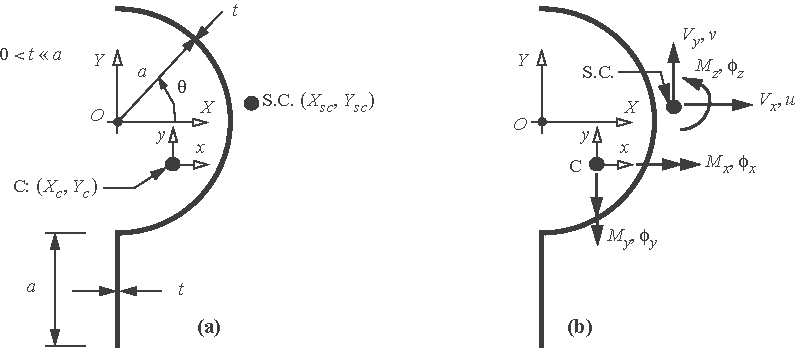
\includegraphics{Figure_3-1.pdf}}{\caption{Thin-walled open cross section: (a) geometry and coordinate systems and (b) internal actions.\label{fig3.1}}}}

\pagebreak
\begin{wrapfigure}[10]{L}{107.67pt}
%\vspace{-19pt}
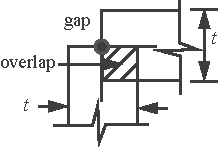
\includegraphics{Figure_3-2.pdf}
\caption{Idealized junction.\label{fig3.2}}
\end{wrapfigure}

The geometry of the bar's cross section is defined by the locus of points along the center line of the wall, which is called the \textbf{contour}, and the thickness $t$ of the wall. The contour consists of piece-wise continuous lines or curves in the plane of the cross section whose subdivisions are called branches. Points between branches occur at junctions or sharp corners. Let the arc-length along the contour be denoted by $s$, and the thickness can be a function of $s$. That is $t=t(s)>0$, as long as it is small with respect to the length of a branch and to its radius of curvature (e.g., $0<t \ll a$ for the section shown in figure~\ref{fig3.1}(a)). At junctions between branches overlaps and gaps of cross-sectional areas can occur as shown in figure~\ref{fig3.2}, but its effect on the geometrical properties of the section are small under the thin-walled assumption. A step change in thickness along a contour is accommodated by defining a junction at the location of\break the step.

The bar is referenced to two, right-handed Cartesian coordinate systems labeled ($X,Y,Z$) and ($x,y,z$). The positive directions of the $Z$-axis and the $z$-axis are out of the plane of the cross section shown in the figure with\break $Z = z$, where $z \in[0, L]$ and $L$ is the axial length of the bar. The cross section shown figure~\ref{fig3.1}(a) is called a positive $z$-face since the normal to the cross section points outward (positive $z$-direction) from the material contained behind the cross section. The origin of the ($X,Y$) system in the cross section is taken at the center of the semicircular branch for convenience, and is labeled point $O$. The ($x,y$) system is parallel to the ($X,Y$) system, and the origin of the ($x,y$) system is at the centroid, which is labeled point $C$. The shear center in the cross section is labeled as point $S.C$.

The internal resultants acting on the cross section of the bar are $N$, $V_{x}$, $V_{y}$, $M_{x}$, $M_{y}$, and $M_{z}$, and these resultants are functions of the axial coordinate $z$. Refer to figure~\ref{fig3.1}(b). The axial normal force is labeled $N$, and is defined positive in tension acting at the centroid. Note that $N$ is not shown in figure~\ref{fig3.1}(b). The axial displacement corresponding to $N$ is denoted by $w(z)$. The transverse shear forces $V_{x}$ and $V_{y}$ are defined positive in positive $x$- and $y$-directions on a positive $z$-face, respectively, and act at the shear center. The displacements corresponding to $V_x$ and $V_y$ are denoted by $u(z)$ and $v(z)$, respectively. The bending moment $M_{x}(z)$ and its corresponding rotation $\phi_{x}(z)$ are referenced to the centroid, and are defined positive in the positive $x$-direction by the right-hand screw rule. (Put your right thumb along the positive $x$-axis and your fingers curl in the direction of the positive moment and corresponding rotation.) The bending moment $M_{y}(z)$ and its corresponding rotation $\phi_{y}(z)$ are referenced to the centroid and are defined positive in the negative $y$-direction by the right-hand screw rule. Note that positive bending moments cause tension of the axial fibers in the first quadrant of the \textit{x-y} coordinate system. The torque is denoted by $M_{z}(z)$, and its corresponding rotation $\phi_{z}(z)$ are defined at the shear center and are positive counterclockwise on the positive $z$-face.


\subsubsection{Centroid C.} The centroid decouples the extension and bending responses of the bar in the material law. Refer to eq.~(\ref{eq3.80}) on page \pageref{eq3.80}. The procedure to locate the centroid is presented in example \ref{ex3.1} on page \pageref{ex3.1} for an open cross-sectional contour, and in part (a) of example \ref{ex3.4} on page \pageref{ex3.4} for a closed cross-sectional contour.

\subsubsection{Shear center S.C.} The shear center is a point in the cross section through which the plane of the loading must pass for the bar to bend and not twist in torsion. That is, the resultant of the shear forces in the cross section must act through the shear center to prevent torsion. Using energy methods in article \ref{sec5.5.3} it is shown that the shear center decouples the transverse shear and torsion responses of the bar in the material law. Refer to eq.~(\ref{eq5.76}) on page \pageref{eq5.76}. The procedure to locate the shear center is presented in example \ref{ex3.3} on page \pageref{ex3.3} for an open cross-sectional contour, and in part (c) of example \ref{ex3.4} on page \pageref{ex3.4} for a closed cross-sectional contour.

\vfill\pagebreak

\section{Contour geometry}\label{sec3.2}

The contour in the cross section is defined in parametric form by its coordinates $x(s)$ and $y(s)$ where $s$ denotes the arc-length of the contour as shown in figure~\ref{fig3.3}(a). The position vector from point $C$ to a point $s$ on the contour is
\begin{align}\label{eq3.1}
\harp{r}(s)=x(s) \hat{i}+y(s) \hat{j},
\end{align}
where the Cartesian unit vectors are denoted $\hat{i}, \hat{j}, \hat{k}$ along the positive $x$-, $y$-, and $z$-directions, respectively. The Cartesian coordinates are a right-handed system, or $\hat{i} \times \hat{j}=\hat{k}$, and the arc-length $s$ is taken positive counter-clockwise along the contour. The differential arc-length on the contour is given by
\begin{align}\label{eq3.2}
d s^{2}=d \harp{r} \bullet d \harp{r}=d x^{2}+d y^{2}, \quad~\text{which implies } \quad\left(\frac{d x}{d s}\right)^{2}+\left(\frac{d y}{d s}\right)^{2}=1.
\end{align}
Unit vectors tangent and normal to the contour are denoted by $\hat{t}(s)$ and $\hat{n}(s)$, respectively. Let the angle between the positive $x$-direction and the unit normal $\hat{n}$ be denoted by $\theta(s)$. From the differential geometry along the contour shown in figure~\ref{fig3.3}, the trigonometric functions of the angle $\theta(s)$ are given by
\begin{align}\label{eq3.3}
\frac{d x}{d s}=-\sin \theta \quad \frac{d y}{d s}=\cos \theta.
\end{align}
{\def\thefigure{3.3}
\processfigure[H]{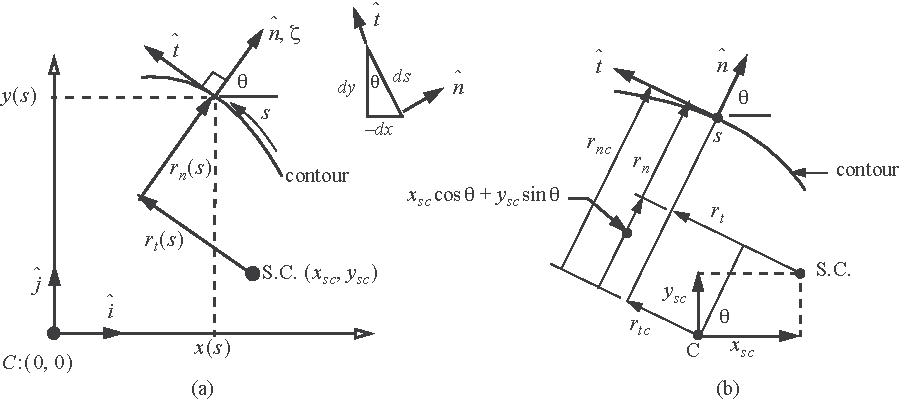
\includegraphics{Figure_3-3.pdf}
}{\caption{(a) Analytic geometry of the contour. (b) Tangential and normal coordinates with respect to the shear center and centroid.\label{fig3.3}}}}
The unit tangent vector to the contour is
\begin{align}\label{eq3.4}
\hat{t}=\frac{d \harp{r}}{d s}=\left(\frac{d x}{d s}\right) \hat{i}+\left(\frac{d y}{d s}\right) \hat{j}=(-\sin \theta) \hat{i}+(\cos \theta) \hat{j}.
\end{align}

\clearpage

\noindent The unit normal to the contour is given by the cross product $\hat{n}=\hat{t} \times \hat{k}$, which yields
\begin{align}\label{eq3.5}
\hat{n}=(\cos \theta) \hat{i}+(\sin \theta) \hat{j}=\left(\frac{d y}{d s}\right) \hat{i}-\left(\frac{d x}{d s}\right) \hat{j}.
\end{align}
The derivatives of the unit tangent and normal vectors along the contour are obtained by differentiating eq.~(\ref{eq3.4}) and eq.~(\ref{eq3.5}) with respect to arc-length $s$. The results are expressed as
\begin{align}\label{eq3.6}
\frac{d \hat{t}}{d s}=\frac{-\hat{n}}{R_{s}} \quad \frac{d \hat{n}}{d s}=\frac{\hat{t}}{R_{s}} \quad \frac{1}{R_{s}}=\frac{d \theta}{d s},
\end{align}
where $d \theta / d s$ is the curvature of the contour at $s$, and $R_{s}$ is the radius of curvature at $s$. For subsequent computations the direction cosines between the two Cartesian and contour unit vectors are listed in table~\ref{tab3.1}

 \begin{table}[!h]%Table 3.1
\processtable{Direction cosines\label{tab3.1}}
{\tabcolsep=12pt\begin{tabular}{@{}llll@{}}
\toprule
 & \colhead{$\hat{i}$} & \colhead{$\hat{j}$} & \colhead{$\hat{k}$}\\
\midrule
$\hat{n}$ & $\cos \theta$ & $\sin \theta$ & $0$\\
$\hat{t}$ & $-\sin \theta$ & $\cos \theta$ & $0$\\
$\hat{k}$ & $0$ & $0$ & $1$\\
\botrule
\end{tabular}}{}
\vspace*{-1pc}
\end{table}

The position vector $\harp{r}(s)$ is also expressed as a function of the tangential coordinate $r_{t}(s)$ and normal coordinate $r_{n}(s)$ by
\begin{align}\label{eq3.7}
\harp{r}(s)=x_{s c} \hat{i}+y_{sc} \hat{j}+r_{t}(s) \hat{t}(s)+r_{n}(s) \hat{n}(s),
\end{align}
where the coordinates of the shear center with respect to the centroid are denoted by $x_{s c}$ and $y_{s c}$. Equating the two expressions (\ref{eq3.1}) and (\ref{eq3.7}) for the position vector and using the direction cosine table 3.1, the following relations between the contour coordinates result:
\begin{gather}\label{eq3.8}
\begin{split}
r_{t}(s)=-\left[x(s)-x_{s c}\right] \sin \theta(s)+\left[y(s)-y_{s c}\right] \cos \theta(s) \\
r_{n}(s)=\left[x(s)-x_{s c}\right] \cos \theta(s)+\left[y(s)-y_{s c}\right] \sin \theta(s)
\end{split}\\
x(s)-x_{s c}=-r_{t}(s) \sin \theta(s)+r_{n}(s) \cos \theta(s) \quad y(s)-y_{s c}=r_{t}(s) \cos \theta(s)+r_{n}(s) \sin \theta(s).\label{eq3.9}
\end{gather}
Replace the trigonometric functions in eq.~(\ref{eq3.8}) by derivatives of the contour coordinates using eq.~(\ref{eq3.3}). Then expand eq.~(\ref{eq3.8}) and write it as
\begin{align}\label{eq3.10}
r_{t}=r_{t c}-x_{s c} \frac{d x}{d s}-y_{s c} \frac{d y}{d s} \quad r_{n}=r_{n c}-x_{s c} \frac{d y}{d s}+y_{s c} \frac{d x}{d s},
\end{align}
where
\begin{align}\label{eq3.11}
r_{t c}=x(s) \frac{d x}{d s}+y(s) \frac{d y}{d s} \quad r_{n c}=x(s) \frac{d y}{d s}-y(s) \frac{d x}{d s}.
\end{align}
In eq.~(\ref{eq3.11}), the tangent and normal coordinates to a generic point on the contour relative to the centroid are denoted by $r_{t c}(s)$ and $r_{n c}(s)$, respectively. The relationship expressed by eq.~(\ref{eq3.10}) is shown in figure~\ref{fig3.3}(b).

\clearpage

The derivative of the position vector with respect to the arc length coordinate $s$ is the unit tangent vector in eq.~(\ref{eq3.4}). Take the derivative of $\harp{r}(s)$ with respect to $s$ using eq.~(\ref{eq3.7}) to get
\begin{align}\label{eq3.12}
\frac{d \harp{r}}{d s}=\hat{t}=\left(\frac{d r_{t}}{d s}+\frac{r_{n}}{R_{s}}\right) \hat{t}+\left(\frac{d r_{n}}{d s}-\frac{r_{t}}{R_{s}}\right) \hat{n}.
\end{align}
Since $d \harp{r} / d s=\hat{t}$, it follows that coordinates $r_{t}(s)$ and $r_{n}(s)$, and the radius of curvature $R_{s}$ are related by
\begin{align}\label{eq3.13}
\frac{d r_{t}}{d s}+\frac{r_{n}}{R_{s}}=1 \quad \frac{d r_{n}}{d s}-\frac{r_{t}}{R_{s}}=0.
\end{align}

\section{Displacements}\label{sec3.3}

Consider a material point in the wall of the cross section located by coordinates ($s,\zeta$), where $\zeta$ denotes the thickness coordinate. Coordinate $\zeta=0$ on the contour and $-t / 2 \leq \zeta \leq t / 2$. Denote the position vector $\harp{R}$ to point ($s,\zeta$) relative to the shear center by
\begin{align}\label{eq3.14}
\harp{R}(s, \zeta)=r_{t} \hat{t}+\left(r_{n}+\zeta\right) \hat{n}.
\end{align}

\removelastskip

\textbf{It is assumed that the cross section displaces, and then undergoes an infinitesimal rotation as a rigid disk.} Let $\harp{u}_{s c}(z)$ denote the displacement vector of the shear center of the cross section, and let $\harp{u}(s,\; z,\; \zeta)$ denote the displacement vector of the particle at point (\textit{s, z, $\zeta$}). The position vector $\harp{R}$ in the cross section is displaced and rotated in the rigid disk to $\harp{R}^{(*)}$. Since $\harp{R}^{(*)}$ is embedded in the rigid disk, the magnitudes of vector $\harp{R}^{(*)}$ and vector $\harp{R}$ are the same; i.e., $\harp{R}^{(*)} \bullet \harp{R}^{(*)}=\harp{R} \bullet \harp{R}$. As shown in figure~\ref{fig3.4} the displacement $\harp{u}(s,\; z,\; \zeta)$ related to displacement $\harp{u}_{s c}(z)$ and the change in direction of vector $\harp{R}$ by
\begin{align}\label{eq3.15}
\harp{u}(s,\; z,\; \zeta)=\harp{u}_{s c}(z)+\harp{R}^{(*)}-\harp{R}.
\end{align}
{\def\thefigure{3.4}
\def\floataboveskip{-12pt}
\processfigure[H]{
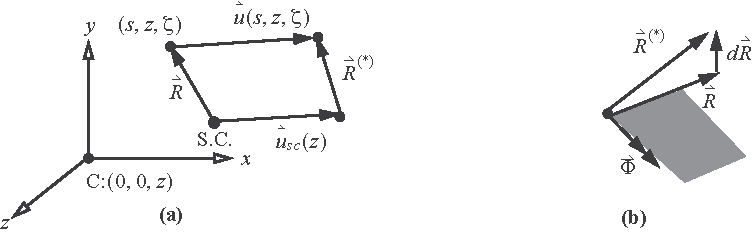
\includegraphics{Figure_3-4.pdf}
}{\caption{(a) Displacement vectors of the shear center and a generic particle in the bar. (b) Change in direction of position vector $\harp{R}$ due to an infinitesimal rotation $\harp{\Phi}$. $d\harp{R}$ is normal to the plane of $\harp{R}$ and $\harp{\Phi}$.\label{fig3.4}}}\vspace*{-12pt}}
\noindent Let $\harp{\Phi}$ denote the infinitesimal rotation vector of the cross section embedded in the rigid disk. The change in direction of $\harp{R}$ is denoted as $d \harp{R}$ and is determined by the vector cross product (Goldstein, p.~\pageref{Goldstein}):
\begin{align}\label{eq3.16}
\harp{R}^{(*)}-\harp{R}=d \harp{R}=\harp{\Phi} \times \harp{R}.
\end{align}
Substitute eq.~(\ref{eq3.16}) for $\harp{R}^{(*)}-\harp{R}$ in eq.~(\ref{eq3.15}) to get
\begin{align}\label{eq3.17}
\harp{u}(s, z, \zeta)=\harp{u}_{s c}(z)+\harp{\Phi} \times \harp{R}.
\end{align}

The vectors $\harp{u}_{sc}(z)$, $\harp{u}(s, z, \zeta)$, and $\bar{\Phi}(z)$ are written in the Cartesian basis or contour coordinate basis as follows:
\begin{gather}
%\begin{split}
\harp{u}_{s c}(z)=u(z) \hat{i}+v(z) \hat{j}+w_{s c}(z) \hat{k} \nonumber\\
\harp{u}(s, z, \zeta)=u_{s}(s, z, \zeta) \hat{t}+u_{z}(s, z, \zeta) \hat{k}+u_{\zeta}(s, z, \zeta) \hat{n} \label{eq3.18}\\
\harp{\Phi}(z)=\phi_{x}(z) \hat{i}-\phi_{y}(z) \hat{j}+\phi_{z}(z) \hat{k},\nonumber
%\end{split},
\end{gather}
where $w_{s c}(z)$ is the axial displacement of the shear center. The components of the displacement vector $\harp{u}(s, z, \zeta)$ in terms of the displacement vector $\harp{u}_{s c}(z)$ of the shear center and the contribution from the rotation is given by the following scalar products:
\begin{align}\label{eq3.19}
%\begin{split}
u_{s}(s, z, \zeta)&=\harp{u}(s, z, \zeta) \bullet \hat{t}=\harp{u}_{s c}(z) \bullet \hat{t}+\harp{\Phi} \times\left(r_{t} \hat{t}+\left(r_{n}+\zeta\right) \hat{n}\right) \bullet \hat{t} \nonumber\\
u_{z}(s, z, \zeta)&=\harp{u}(s, z, \zeta) \bullet \hat{k}=\harp{u}_{s c}(z) \bullet \hat{k}+\harp{\Phi} \times\left(r_{t} \hat{t}+\left(r_{n}+\zeta\right) \hat{n}\right) \bullet \hat{k} \\
u_{\zeta}(s, z, \zeta)&=\harp{u}(s, z, \zeta) \bullet \hat{n}=\harp{u}_{s c}(z) \bullet \hat{n}+\harp{\Phi} \times\left(r_{t} \hat{t}+\left(r_{n}+\zeta\right) \hat{n}\right)\bullet \hat{n}.\nonumber
%\end{split}.
\end{align}
Performing the scalar products in eq.~(\ref{eq3.19}) with the aid of (\ref{eq3.9}) and (\ref{eq3.18}) and table 3.1, we find that the displacement components of a particle in the cross section with respect to the shear center are
\begin{gather}
u_{s}(s, z, \zeta)=-u(z) \sin \theta(s)+v(z) \cos \theta(s)+\left[r_{n}(s)+\zeta\right] \phi_{z}(z),\label{eq3.20}\\
u_{z}(s, z, \zeta)=w_{s c}(z)+\left[y(s)-y_{s c}\right] \phi_{x}(z)+\left[x(s)-x_{s c}\right] \phi_{y}(z)+\zeta\left[\phi_{x}(z) \sin \theta(s)+\phi_{y}(z) \cos \theta(s)\right],\label{eq3.21}\\
u_{\zeta}(s, z, \zeta)=u(z) \cos \theta(s)+v(z) \sin \theta(s)-r_{t}(s) \phi_{z}(z).\label{eq3.22}
\end{gather}

\removelastskip

Let $\harp{u}_{c}(z)$ denote the displacement of the centroid, with the component form given by
\begin{align}\label{eq3.23}
\harp{u}_{c}(z)=u_{c}(z) \hat{i}+v_{c}(z) \hat{j}+w(z) \hat{k}.
\end{align}
where $u_{c}(z)$ and $v_{c}(z)$ denote the $x$-direction and $y$-direction displacements of the centroid. From figure~\ref{fig3.5} the displacement of the shear center relative to the displacement of the centroid is
\begin{align}\label{eq3.24}
\harp{u}_{s c}(z)=\harp{u}_{c}(z)+\harp{R}_{s c}^{*}-\harp{R}_{s c}=\harp{u}_{c}(z)+d \harp{R}_{s c}=\harp{u}_{c}(z)+\harp{\Phi} \times \harp{R}_{s c}.
\end{align}

\vspace*{-1.2pc}

\begin{wrapfigure}[10]{L}{135.5pt}\vspace*{-15pt}
\includegraphics{Figure_3-5.pdf}
\caption{Displacements of the centroid and shear center.\label{fig3.5}}
\end{wrapfigure}

\noindent where it is noted that position vector $\harp{R}_{s c}$ is embedded in the rigid disk containing the cross section which undergoes the infinitesimal rotation $\harp{\Phi}(z)$. Position vector $\harp{R}_{s c}=x_{s c} \hat{i}+y_{s c} \hat{j}$, and the rotation vector is given in eq.~(\ref{eq3.18}). From the forgoing vector relations, the displacement components of the shear center relative to the centroid are
\begin{gather}\label{eq3.25}
\begin{split}
u(z)&=u_{c}(z)-y_{s c} \phi_{z}(z) \\
v(z)&=v_{c}(z)+x_{s c} \phi_{z}(z) \\
w_{s c}(z)&=w(z)+x_{s c} \phi_{y}(z)+y_{s c} \phi_{x}(z)
\end{split}.
\end{gather}

\removelastskip

Substitute the expression for axial displacement $w_{s c}(z)$ from eq.~(\ref{eq3.25}) into eq.~(\ref{eq3.21}) to get
\begin{align}\label{eq3.26}
u_{z}(s, z, \zeta)=w(z)+y(s) \phi_{x}(z)+x(s) \phi_{y}(z)+\zeta\left[\phi_{x}(z) \sin \theta(s)+\phi_{y}(z) \cos \theta(s)\right].
\end{align}

\clearpage

\section{Strains}\label{sec3.4}\enlargethispage{-1\baselineskip}

Consider three mutually perpendicular, infinitesimal line elements $dS$, \textit{dz}, and $d\zeta$ in the undeformed body, where the arc-length of the line element parallel to the contour is related to the arc-length of the contour by $dS=\left(1+\zeta / R_{s}\right) ds$. Let $\varepsilon_{ss}$ denote the normal strain for line element \textit{dS}, $\boldsymbol{\varepsilon}_{zz}$ the normal strain for \textit{dz}, and $\varepsilon_{\zeta \zeta}$ the normal strain for line element $d\zeta$. For infinitesimal deformations, these normal strains are related to displacements $u_s$, $u_z$, and $u_{\zeta}$ by\vspace*{-8pt}
\begin{align}\label{eq3.27}
\varepsilon_{s s}=\left(\frac{\partial u_{s}}{\partial s}+\frac{u_{\zeta}}{R_{s}}\right) /\left(1+\frac{\zeta}{R_{s}}\right) \quad \varepsilon_{z z}=\frac{\partial u_{z}}{\partial z} \quad \varepsilon_{\zeta \zeta}=\frac{\partial u_{\zeta}}{\partial \zeta}.
\end{align}
Let $\gamma_{z s}$ denote the engineering shear strain between line elements \textit{dS} and \textit{dz}, $\gamma_{s \zeta}$ the engineering shear strain between \textit{dS} and $d\zeta$, and $\gamma_{z \zeta}$ the engineering shear strain between line elements \textit{dz} and $d\zeta$. For infinitesimal deformations, the shear strain-displacement relations are
\begin{align}\label{eq3.28}
\gamma_{z s}=\frac{\partial u_{s}}{\partial z}+\frac{1}{\left(1+\zeta / R_{s}\right)} \frac{\partial u_{z}}{\partial s} \quad \gamma_{s \zeta}=\frac{\partial u_{s}}{\partial \zeta}+\frac{1}{\left(1+\zeta / R_{s}\right)}\left(\frac{\partial u_{\zeta}}{\partial s}-\frac{u_{s}}{R_{s}}\right) \quad \gamma_{z \zeta}=\frac{\partial u_{z}}{\partial \zeta}+\frac{\partial u_{\zeta}}{\partial z}.
\end{align}

\removelastskip

Substitute the displacements from eqs. (\ref{eq3.20}), (\ref{eq3.22}), and (\ref{eq3.26}) into the strain-displacement relations for $\varepsilon_{ss}$, $\mathcal{\varepsilon}_{\zeta \zeta}$ and $\gamma_{s} \zeta$, to find
\begin{align}\label{eq3.29}
\varepsilon_{s s}=\frac{\left(\frac{d r_{n}}{d s}-\frac{r_{t}}{R_{s}}\right)}{1+\zeta / R_{s}} \phi_{z}=0 \quad \varepsilon_{\zeta \zeta}=0 \quad \gamma_{s \zeta}=\left[1-\frac{\left(\frac{d r_{t}}{d s}+\frac{r_{n}}{R_{s}}+\frac{\zeta}{R_{s}}\right)}{1+\frac{\zeta}{R_{s}}}\right] \phi_{z}=0.
\end{align}
Strains $\varepsilon_{s s}=\gamma_{s \zeta}=0$ result from the relations between the coordinates $r_{n}$ and $r_{t}$ given by eq.~(\ref{eq3.13}). Moreover, the vanishing of the strains in eq.~(\ref{eq3.29}) is a consequence of the assumption that the cross section is undeformable in its own plane. Substitute the axial displacement from eq.~(\ref{eq3.26}) into the axial normal strain-displacement in eq.~(\ref{eq3.27}) to get
\begin{align}\label{eq3.30}
\varepsilon_{z z}=\frac{d w}{d z}+y(s) \frac{d \phi_{x}}{d z}+x(s) \frac{d \phi_{y}}{d z}+\zeta\left[\frac{d \phi_{x}}{d z} \sin \theta(s)+\frac{d \phi_{y}}{d z} \cos \theta(s)\right].
\end{align}
Substitute the displacements from eqs. (\ref{eq3.20}), (\ref{eq3.22}), and (\ref{eq3.26}) into the last two shear strain-displacement equations to find
\begin{align}\label{eq3.31}
\gamma_{z s}=-\psi_{x} \sin \theta+\psi_{y} \cos \theta+\left(r_{n}(s)+\zeta\right) \frac{d \phi_{z}}{d z} \quad \gamma_{z \zeta}=\psi_{x} \cos \theta+\psi_{y} \sin \theta-r_{t} \frac{d \phi_{z}}{d z}.
\end{align}
In previous expressions for the shear strains new quantities $\psi_{x}$ and $\psi_{y}$ are introduced. These new quantities represent shear strains averaged over the cross section of the bar and are defined by
\begin{align}\label{eq3.32}
\psi_{x}(z)=\frac{d u}{d z}+\phi_{y}(z) \quad \psi_{y}(z)=\frac{d v}{d z}+\phi_{x}(z).
\end{align}
See figure~\ref{fig3.6} for a graphical representation of these averaged transverse shear strains.


{\def\thefigure{3.6}
\processfigure[H]{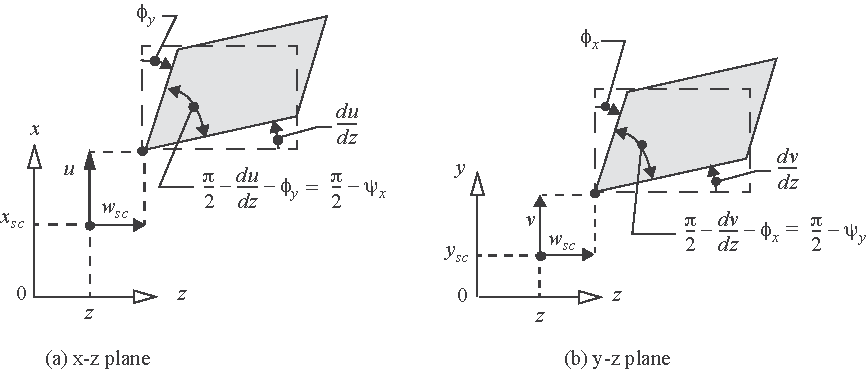
\includegraphics{Figure_3-6.pdf}
}{\caption{Transverse shear strains of the bar with respect to the shear center: (a) projection in the $x$-$z$ plane, (b) projection in the $y$-$z$ plane.\label{fig3.6}}}}

\section{Stresses, stress resultants and bar resultants}\label{sec3.5}

Let $\sigma_{z z}$ denote the stress normal to the cross section, $\sigma_{z s}$ denote the shear stress acting tangent to the contour of the cross section, and let $\sigma_{z \zeta}$ denote the shear stress normal to the contour acting on the cross section. These stress components act on an infinitesimal area of the cross section denoted by $d A=\left(1+\zeta / R_{s}\right) d s d \zeta$.These stress components\enlargethispage{-3\baselineskip} are shown in figure~\ref{fig3.7}(a).

{\def\thefigure{3.7}
\processfigure[H]{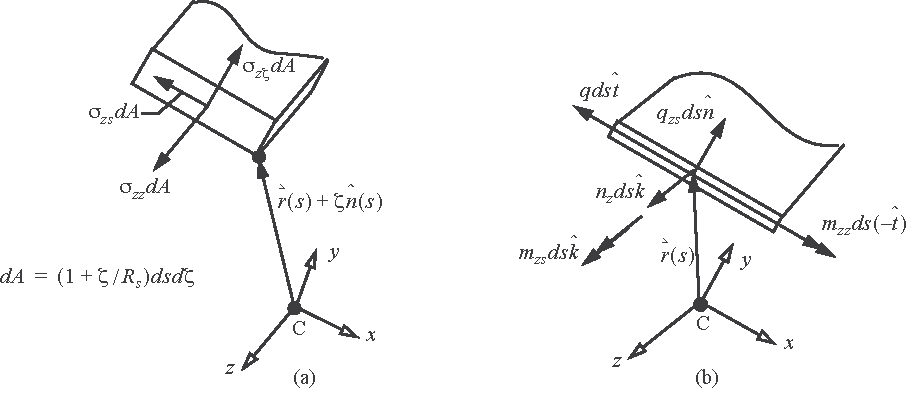
\includegraphics{Figure_3-7.pdf}
}{\caption{(a) Stress components acting on differential area $dA$ of the cross section. (b) stress resultants acting at the contour of length $ds$.\label{fig3.7}}}}

Consider the work done on a cross section at a fixed value of $z$ by the stresses acting through incremental displacements. The incremental displacement corresponding to $\sigma_{z z}$ is $\delta u_{z}$\footnote{The notation $\delta u_z$ denotes a continuos function of infinitesimal magnitude added to the displacement function $u_z$, which vanishes at prescribed values of $u_z$. That is, $u_z+\delta u_z$ is a new displacement function. Function $\delta u_z$ is interpreted as a change in displacement at fixed values of independent coordinates $s$, $z$, and $\zeta$, where the independent variables identify a material point. In differential calculus $d u_z$ is the infinitesimal change in the displacement function with respect to changes in the independent variables without changing the function itself.}, incremental displacement corresponding to $\sigma_{z s}$ is $\delta u_{s}$, and the incremental displacement corresponding to $\sigma_{z \zeta}$ is $\delta u_{\zeta}$. Let $\delta W_{z}$ denote the incremental work, which is given by the integral
\begin{align}\label{eq3.33}
\delta W_{z}=\int_{c}\left[\int_{-t / 2}^{t / 2}\left(\sigma_{z z} \delta u_{z}+\sigma_{z s} \delta u_{s}+\sigma_{z \zeta} \delta u_{\varepsilon}\right)\left(1+\zeta / R_{s}\right) d \zeta\right] d s.
\end{align}
The incremental displacements are determined from eqs. (\ref{eq3.20}), (\ref{eq3.22}), and (\ref{eq3.26}), and are
\begin{align}\label{eq3.34}
\begin{split}
\delta u_{z}(s, z, \zeta)&=\delta w(z)+y(s) \delta \phi_{x}(z)+x(s) \delta \phi_{y}(z)+\zeta\left[\delta \phi_{x}(z) \sin \theta(s)+\delta \phi_{y}(z) \cos \theta(s)\right] \\
\delta u_{s}(s, z, \zeta)&=-\delta u(z) \sin \theta(s)+\delta v(z) \cos \theta(s)+\left[r_{n}(s)+\zeta\right] \delta \phi_{z}(z) \\
\delta u_{\zeta}(s, z, \zeta)&=\delta u(z) \cos \theta(s)+\delta v(z) \sin \theta(s)-r_{t}(s) \delta \phi_{z}(z)
\end{split},
\end{align}
where $\delta u(z)$, $\delta v(z)$, and $\delta w(z)$ denote the incremental displacements of the cross section, $\delta \phi_{x}(z)$, $\delta \phi_{y}(z)$, and $\delta \phi_{z}(z)$ denote the incremental rotations of the cross section. Substitute the incremental displacements from eq.~(\ref{eq3.34}) into the expression (\ref{eq3.33}) for the incremental work, followed by integration through the thickness of the wall. The result of this process is written as
\begin{align}
\delta W_{z}=& \int_{c}\left[\left(-q \sin \theta+q_{z} \cos \theta\right) \delta u+\left(q \cos \theta+q_{z} \sin \theta\right) \delta v+n_{z} \delta w\right.\nonumber\\
&+\left.\left(y n_{z}+m_{z z} \sin \theta\right) \delta \phi_{x}+\left(x n_{z}+m_{z z} \cos \theta\right) \delta \phi_{y}+\left(r_{n} q+m_{z s}-r_{t} q_{z}\right) \delta \phi_{z}\right] d s.\label{eq3.35}
\end{align}
The integration through the thickness leads to the definition of stress resultants acting at the contour. The normal stress resultant is denoted by $n_{z}$, shear flow resultant by \textit{q, }transverse stress resultant by $q_{z}$, bending moment resultant by $m_{z}$, and twisting moment resultant by $m_{z s}$. These stress resultants are given by the following integrals through the thickness:
\begin{align}\label{eq3.36}
\left(n_{z}, m_{z}\right)=\int_{-t / 2}^{t / 2}(1, \zeta) \sigma_{z z}\left(1+\zeta / R_{s}\right) d \zeta,
\end{align}
and
\begin{align}\label{eq3.37}
\left(q, m_{z s}\right)=\int_{-t / 2}^{t / 2}(1, \zeta) \sigma_{z s}\left(1+\zeta / R_{s}\right) d \zeta \quad q_{z}=\int_{-t / 2}^{t / 2} \sigma_{z \zeta}\left(1+\zeta / R_{s}\right) d \zeta.
\end{align}
See figure~\ref{fig3.7}(b).

The integral over the contour of the incremental work in (\ref{eq3.35}) is written as
\begin{align}\label{eq3.38}
\delta W_{z}=V_{x} \delta u+V_{y} \delta v+N \delta w+M_{x} \delta \phi_{x}+M_{y} \delta \phi_{y}+M_{z} \delta \phi_{z}.
\end{align}
Integration over the contour defines the bar resultants in terms of the stress resultants as
\begin{gather}
N=\int_{c} n_{z} d s \quad M_{x}=\int_{c}\left(y n_{z}+m_{z z} \sin \theta\right) d s \quad M_{y}=\int_{c}\left(x n_{z}+m_{z z} \cos \theta\right) d s,
\mbox{ and}\label{eq3.39}\\
V_{x}=\int_{c}\left(-q \sin \theta+q_{z} \cos \theta\right) d s \quad V_{y}=\int_{c}\left(q \cos \theta+q_{z} \sin \theta\right) d s \quad M_{z}=\int_{c}\left(r_{n} q+m_{z s}-r_{t} q_{z}\right) d s.\label{eq3.40}
\end{gather}



\section{External loads and equilibrium of an element of the bar}\label{sec3.6}

The prescribed external traction components acting on the bar are denoted by functions $p_{n}(s, z)$, $p_{s}(s, z)$ and $p_{z}(s, z)$, which are defined per unit area of the middle surface where $\zeta=0$. The dimensional units of these traction components are ${F/L}^2$. See figure~\ref{fig3.8}. At a typical cross section these tractions are resolved into distributed line loads $f_{x}$, $f_{y}$ and $f_{z}$ having dimensional units \textit{F/L}. The line loads are determined from the following vector\break relation:
\begin{align}\label{eq3.41}
\harp{f}(z)=f_{x} \hat{i}+f_{y} \hat{j}+f_{z} \hat{k}=\int_{c}(p_{n} \hat{n}+p_{s} \hat{t}+p_{z} \hat{k}) d s.
\end{align}
Using the direction cosines in table 3.1, these line load intensities are related to the specified tractions by
{\def\thefigure{3.8}
\processfigure[H]{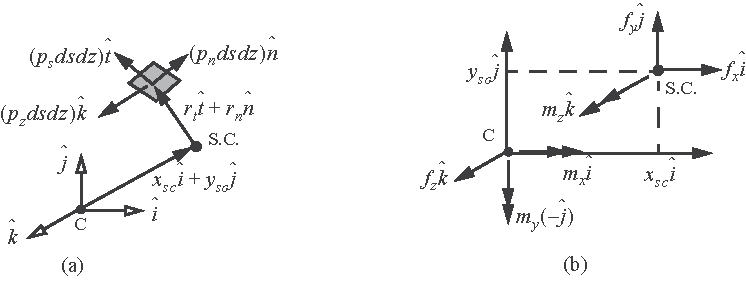
\includegraphics{Figure_3-8.pdf}
}{\caption{(a) External tractions prescribed on the reference surface. (b) Statically equivalent external line load intensities.\label{fig3.8}} \def\floatbelowskip{-24pt}}}

\vspace*{-3pc}

\begin{align}\label{eq3.42}
f_{x}(z)=\int_{c}\left(p_{n} \cos \theta-p_{s} \sin \theta\right) d s \quad f_{y}(z)=\int_{c}\left(p_{n} \sin \theta+p_{s} \cos \theta\right) d s \quad f_{z}(z)=\int_{c} p_{z} d s.
\end{align}
At a typical cross section these traction components result in an external torque per unit axial length with respect to the centroid denoted by $\left.\bar{m}_{z}\right|_{C}$, with dimensional units (\textit{F-L/)L. }The external moment per unit axial length with respect to centroid is determined from the following vector cross product relation:
\begin{align}\label{eq3.43}
\harp{m}_{C}=\int_{c}\left[(x_{s c} \hat{i}+y_{sc} \hat{j})+(r_{n} \hat{n}+r_{t} \hat{t} )\right] \times\left[p_{n} \hat{n}+p_{s} \hat{t}+p_{z} \hat{k}\right] d s.
\end{align}
Perform the cross products to find the moment per unit axial length about the centroid from the prescribed traction to get
\begin{align}\label{eq3.44}
\harp{m}_{C} =m_{x} \hat{i}-m_{y} \hat{j}+\left[x_{sc} f_{y}(z)-y_{sc} f_{x}(z)+m_{z}(z)\right] \hat{k},
\end{align}
where
\begin{align}\label{eq3.45}
m_{x}=\int_{c} y(s) p_{z}(s, z) d s \quad m_{y}=\int_{c} x(s) p_{z}(s, z) d s \quad m_{z}=\int_{c}\left[r_{n}(s) p_{s}(s, z)-r_{t}(s) p_{n}(s, z)\right] d s,
\end{align}

\removelastskip

Equation (\ref{eq3.38}) is applicable at each end of the bar where $z = 0$ and $z = L$. Hence, $[N, w]$, $[V_{x}, u]$, $[V_{y}, v]$, $[M_{x}, \phi_{x}]$, $[M_{y}, \phi_{y}]$, and $[M_{z}, \phi_{z}]$ are corresponding variables. We can prescribe a ``force'' variable or its \text{corresponding} ``displacement'' variable as external ``loads'' acting on the end cross sections, but not both the ``force'' and the ``displacement'' simultaneously.

\subsection{Differential equilibrium equations}\label{sec3.6.1}

Let the internal forces acting on the cross section at $z$ be denoted by the vector $\harp{F}(z)$, and let the internal moments acting on the cross section resolved at the centroid be denoted by the vector $\harp{M}(z)$. These vectors of internal actions~are
\begin{align}
\harp{F}(z)=V_{x} \hat{i}+V_{y} \hat{j}+N \hat{k}\mbox{, and}\label{eq3.46}\\
\harp{M}(z)=M_{x} \hat{i}-M_{y} \hat{j}+M_{z C} \hat{k}.\label{eq3.47}
\end{align}
Consider the forces and moments acting on a bar element defined by $z$ and $z+ \Delta z$, $\Delta z>0$, as shown in figure~\ref{fig3.9}.

{\def\thefigure{3.9}
\processfigure[H]{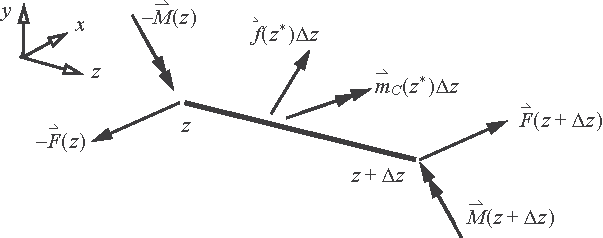
\includegraphics{Figure_3-9.pdf}
}{\caption{A free body diagram of the segment $\Delta z$ of a bar subject to internal actions at its end cross sections, and subject to prescribed external actions along its length.\label{fig3.9}}}}

The vector equations of equilibrium are
\begin{align}\label{eq3.48}
\harp{F}(z+\Delta z)-\harp{F}(z)+\harp{f}\left(z^{*}\right) \Delta z=0 \quad \harp{M}(z+\Delta z)-\harp{M}(z)+\Delta z \hat{k} \times \harp{F}(z+\Delta z)+\left(z^{*}-z\right) \hat{k} \times \harp{f}\left(z^{*}\right) \Delta z+ \harp{m}_{C}\left(z^{*}\right)=0,
\end{align}
where $z<z^{*}<z+\Delta z$. For a continuous force vector and moment vector with respect to coordinate $z$, eq.~(\ref{eq3.48}) can be written as
\begin{align}\label{eq3.49}
\left.\frac{d \harp{F}}{d z}\right|_{z} \Delta z+\harp{f}\left(z^{*}\right) \Delta z=\left.0 \quad \frac{d \harp{M}}{d z}\right|_{z} \Delta z+\Delta z \hat{k} \times \harp{F}(z+\Delta z)+\left(z^{*}-z\right) \hat{k} \times \harp{f}\left(z^{*}\right) \Delta z+\harp{m}_{C}\left(z^{*}\right) \Delta z=0.
\end{align}
Divide the latter equations by $\Delta z$ and take the limit as $\Delta z \rightarrow 0$ and note that $z^{*} \rightarrow z$ in the limit. The differential equations of equilibrium obtained from the limiting procedure are
\begin{align}\label{eq3.50}
\frac{d \harp{F}}{d z}+\harp{f}(z)=0 \quad \frac{d \harp{M}}{d z}+\hat{k} \times \harp{F}(z)+\harp{m}_{C}(z)=0.
\end{align}
Expand the differential equation (\ref{eq3.50}) in terms of components to get
\begin{align}
\left(\frac{d V_{x}}{d z}+f_{x}\right) \hat{i}+\left(\frac{d V_{y}}{d z}+f_{y}\right) \hat{j}+\left(\frac{d N}{d z}+f_{z}\right) \hat{k}=0 \hat{i}+0 \hat{j}+0 \hat{k}\mbox{, and}\label{eq3.51}\\
\left(\frac{d M_{x}}{d z}-V_{y}+m_{x}\right) \hat{i}+\left(-\frac{d M_{y}}{d z}+V_{x}-m_{y}\right) \hat{j}+\left(\frac{d M_{z C}}{d z}+m_{z}+x_{sc} f_{y}-y_{sc} f_{x}\right) \hat{k}=0 \hat{i}+0 \hat{j}+0 \hat{k}.\label{eq3.52}
\end{align}

\subsubsection{Axial equilibrium.} From $\hat{k}$-component of eq.~(\ref{eq3.51}) the differential equilibrium equation is
\begin{align}\label{eq3.53}
\frac{d N}{d z}+f_{z}(z)=0 \quad N=N(z) \quad 0<z<L.
\end{align}

\vspace*{-10pt}\pagebreak

\noindent At the end points $z$ = 0 and $z$ = $L$, prescribe either axial force $N$ or the corresponding displacement $w$, but not both.

\subsubsection{Bending in the \textit{y-z} plane.} From the $\hat{j}$ component of eq.~(\ref{eq3.51}) the differential equation for the shear force is
\begin{align}\label{eq3.54}
\frac{d V_{y}}{d z}+f_{y}(z)=0 \quad V_{y}=V_{y}(z) \quad 0<z<L.
\end{align}
At the end points $z$ = 0 and $z$ = $L$, prescribe either shear force $V_y$ or the corresponding displacement $v$, but not both. From the $\hat{i}$-component of eq.~(\ref{eq3.52}) the differential equation for the bending moment is
\begin{align}\label{eq3.55}
\frac{d M_{x}}{d z}-V_{y}+m_{x}(z)=0 \quad M_{x}=M_{x}(z) \quad 0<z<L.
\end{align}
At the end points $z = 0$ and $z=L$, prescribe either bending moment $M_{x}$ or the corresponding rotation $\phi_{x}$, but not both.

\subsubsection{Bending in the \textit{x-z} plane.} From the $\hat{i}$-component of eq.~(\ref{eq3.51}) the differential equation for the shear force is
\begin{align}\label{eq3.56}
\frac{d V_{x}}{d z}+f_{x}(z)=0 \quad V_{x}=V_{x}(z) \quad 0<z<L.
\end{align}
At the end points $z$ = 0 and $z$ = $L$, prescribe either shear force $V_x$ or the corresponding displacement $u$, but not both. From the $\hat{j}$-component of eq.~(\ref{eq3.52}) the differential equation for the bending moment is
\begin{align}\label{eq3.57}
\frac{d M_{y}}{d z}-V_{x}+m_{y}(z)=0 \quad M_{y}=M_{y}(z) \quad 0<z<L.
\end{align}
At the end points $z = 0$ and $z = L$, prescribe either bending moment $M_y$ or the corresponding rotation $\phi_{y}$, but not both.

\subsubsection{Torsion.} From the $\hat{k}$-component of eq.~(\ref{eq3.52}) the differential equation for torsion about the centroid  is
\begin{align}\label{eq3.58}
\frac{d M_{z C}}{d z}+x_{sc} f_{y}-y_{sc} f_{x}+m_{z}=0.
\end{align}
The torque at the centroid is related to the torque and the shear forces acting at the shear center by static equivalence. (Refer to Fig. \ref{fig3.23} on page \pageref{fig3.23}.) That is,
\begin{align}\label{eq3.59}
M_{z C}=M_{z}+x_{s c} V_{y}-y_{s c} V_{x}.
\end{align}
Substitute eq.~(\ref{eq3.59}) for $M_{z C}$ into eq.~(\ref{eq3.58}) to get
\begin{align}\label{eq3.60}
\frac{d M_{z}}{d z}+x_{s c}\left(\frac{d V_{y}}{d z}+f_{y}\right)-y_{s c}\left(\frac{d V_{x}}{d z}+f_{z}\right)+m_{z}=0.
\end{align}
Impose equilibrium eqs. (\ref{eq3.54}) and (\ref{eq3.56}) in eq.~(\ref{eq3.60}) to get
\begin{align}\label{eq3.61}
\frac{d M_{z}}{d z}+m_{z}=0 \quad M_{z}=M_{z}(z) \quad 0<z<L.
\end{align}
At the end points $z = 0$ and $z=L$, prescribe either torque $M_z$ or the corresponding rotation $\phi_{z}$, but not both\vspace*{6pt}.

\clearpage

\section{Hooke's law}\label{sec3.7}

For a linear elastic, isotropic material, there are two independent material constants: the modulus of elasticity $E$ and Poisson's ratio $\nu$. (Refer to eq. (\ref{eqA.146}) in the appendix.) Hooke's law for the normal strains is
\begin{align}\label{eq3.62}
\left[\begin{array}{@{}l@{}}
\varepsilon_{s s} \\
\varepsilon_{z z} \\
\varepsilon_{\zeta \zeta}
\end{array}\right]=\left[\begin{array}{@{}ccc@{}}1 / E & -v / E & -v / E \\-v / E & 1 / E & -v / E \\-v / E & -v / E & 1 / E\end{array}\right]\left[\begin{array}{@{}l@{}}\sigma_{s s} \\\sigma_{z z} \\\sigma_{\zeta \zeta}\end{array}\right],
\end{align}
where $\sigma_{ss}$ denotes the normal stress acting on the $s$-face, and where $\sigma_{\zeta \zeta}$ denotes the normal stress on the $\zeta$-face acting on an infinitesimal element \textit{ds}-by-\textit{dz}-by-$d\zeta$. The thickness normal stress $\sigma_{\zeta \zeta}$ is assumed to be very small with respect to the axial normal stress $\sigma_{z z}$, and hence is neglected in Hooke's law. From the kinematic assumption, eq.~(\ref{eq3.29}), the normal strain $\varepsilon_{\zeta \zeta}=0$. Setting $\varepsilon_{\zeta \zeta}=\sigma_{\zeta \zeta}=0$ in the third row of eq.~(\ref{eq3.62}), leads to $\sigma_{s s} +\sigma_{z z}=0$, which is a very unlikely result. Thus, we neglect this third equation in Hooke's law. Furthermore, in most thin-walled beam theories (e.g., see Gjelsvik, 1981, p. 16), the normal stress $\sigma_{ss}$ is assumed to be small with respect to the axial normal stress $\sigma_{z z}$ and is neglected in Hooke's law. Setting $\sigma_{ss}=\sigma_{\zeta \zeta}=0$ leads to
\begin{align}\label{eq3.63}
\sigma_{z z}=E \varepsilon_{z z}.
\end{align}
Consequently, the first row of matrix eq.~(\ref{eq3.62}) leads to $\varepsilon_{ss}=-\nu \sigma_{z z} / E$. However, the kinematic assumption, eq.~(\ref{eq3.29}), resulted in $\varepsilon_{s s}=0$. If we set $\varepsilon_{ss}=0$ in the first row of eq.~(\ref{eq3.62}), solve it for $\sigma_{ss}$, followed by substitution into the second row of eq.~(\ref{eq3.62}), we get
\begin{align}\label{eq3.64}
\sigma_{z z}=\frac{E}{1-v^{2}} \varepsilon_{z z}.
\end{align}
It is recognized that Hooke's law in the elasticity sense of eq.~(\ref{eq3.62}) is violated under the assumptions of the thin-walled beam theory under consideration. In the following developments of the theory, eq.~(\ref{eq3.63}) is assumed as the material law governing the axial normal stress and axial normal strain, which is a common assumption in classical beam theory.

\subsection{Effect of thermal expansion}\label{sec3.7.1}

Consider structures subject not only to external forces, but also subject to heating. Aerospace examples include high-speed flight vehicles and orbiting space structures. Aerothermal loads consisting of pressure, skin friction or shearing stresses, and aerodynamic heating, are exerted on the external surfaces of high-speed flight vehicles. Conduction and radiant heat transfer result in significant thermally induced forces acting on orbiting space structures. These aerospace examples are discussed in detail by Thornton (1996), who provides an historical account, and methods of analysis, of thermal structures for aerospace applications.

It is assumed that a change in temperature (thermal state) causes a change in deformation and stress (mechanical state) in the structure, but a change in deformation does not cause a change in temperature. For example, under adiabatic conditions strain can cause a change in temperature. However, in many structural applications the change in temperature under adiabatic straining is negligible and can be ignored (Fung, 1965, p. 390). Thornton (1996, p.51) defines the change in thermal energy state causing a change in mechanical state, but not the reverse, as one-way thermal-mechanical coupling. Thus, heat conduction and thermoelasticty separate into two separate problems. In this text it is assumed that the heat conduction problem has been solved so that the temperature distribution in the structure is known. The \textbf{thermoelastic problem} is to determine the mechanical state in an elastic structure for the specified temperature distribution and the specified external loads.

For a uniaxial stress state the generalized Hooke's law including temperature is
\begin{align}\label{eq3.65}
\varepsilon_{z z}=\left(\sigma_{z z}+\beta \Delta T\right) / E \quad~\text{or } \quad \sigma_{z z}=E \varepsilon_{z z}-\beta \Delta T,
\end{align}
where $\beta=E \alpha$, and $\alpha$ is the coefficient of thermal expansion. The change in temperature is denoted by $\Delta T=T-T_{0}$, and $T_{0}$ is the spatially uniform temperature in the reference state. The reference state is stress free when the external loads acting on the bar are removed and the spatially uniform temperature $T=T_{0}$. Assume a linear distribution of the change in temperature in the thickness, which we write as
\begin{align}\label{eq3.66}
\Delta T(s, z, \zeta)=\Delta T(s, z)+\zeta D T(s, z),
\end{align}
where
\begin{align}\label{eq3.67}
\Delta T(s, z)=\Delta T(s, z, 0) \quad~\text{and } \quad D T(s, z)=\left.\frac{\partial \Delta T}{\partial \zeta}\right|_{\zeta=0}.
\end{align}

\subsection{Material law for extension and bending}\label{sec3.7.2}

Substitute the expression (\ref{eq3.30}) for the axial strain, and substitute eq.~(\ref{eq3.66}) for the change in temperature, into Hooke's law (\ref{eq3.65}) to get the following expression for normal stress.
\begin{align}\label{eq3.68}
\sigma_{z z}=E\left[\frac{d w}{d z}+y(s) \frac{d \phi_{x}}{d z}+x(s) \frac{d \phi_{y}}{d z}-\alpha \Delta T(s, z)\right]+\zeta E\left[\frac{d \phi_{x}}{d z} \sin \theta(s)+\frac{d \phi_{y}}{d z} \cos \theta(s)-\alpha D T(s, z)\right].
\end{align}
\textbf{In the thin-wall bar theory we neglect the distribution of the normal stress and normal strain across the thickness of the wall.} Therefore, the normal strain and stress is assumed uniform in the thickness coordinate, and are given by
\begin{gather}
\varepsilon_{z z}=\frac{d w}{d z}+y(s) \frac{d \phi_{x}}{d z}+x(s) \frac{d \phi_{y}}{d z}\mbox{, and}\label{eq3.69}\\
\sigma_{z z}=E\left[\frac{d w}{d z}+y(s) \frac{d \phi_{x}}{d z}+x(s) \frac{d \phi_{y}}{d z}-\alpha \Delta T(s, z)\right].\label{eq3.70}
\end{gather}
In other words, the local bending of the wall represented by the bending moment resultant $m_{zz}$ in (\ref{eq3.36}) is neglected with respect to the membrane stiffness of the wall represented by the normal stress resultant $n_z$. In addition, for a thin, curved wall we neglect the term $\zeta / R_{s}$ in the factor $\left(1+\zeta / R_{s}\right)$ appearing in the integrand of eq.~(\ref{eq3.36})\footnote{Note that $|\zeta/R_s|\leq |t/(2R_s)|$. A contour that is a straight line has $1/R_s=0$. A thin, curved wall is one in which $R_s>10t$. Hence, $0\leq |t/(2R_s)|<0.05$ for most practical contour geometries\vspace*{4pt}.}. The definition of the normal stress resultant reduces to
\begin{align}\label{eq3.71}
n_{z}=\int_{-t / 2}^{t / 2} \sigma_{z z} d \zeta.
\end{align}
Substitute eq.~(\ref{eq3.70}) for the normal stress into the normal stress resultant (\ref{eq3.71}) to get
\begin{align}\label{eq3.72}
n_{z}=E t\left[\frac{d w}{d z}+y(s) \frac{d \phi_{x}}{d z}+x(s) \frac{d \phi_{y}}{d z}-\alpha \Delta T(s, z)\right].
\end{align}

The constitutive equation for the axial normal force $N$ is obtained by substituting eq.~(\ref{eq3.72}) for the normal stress resultant in the expression (\ref{eq3.39}). The result is
\begin{align}\label{eq3.73}
N=E A \frac{d w}{d z}+E Q_{x} \frac{d \phi_{x}}{d z}+E Q_{y} \frac{d \phi_{y}}{d z}-N_{T},
\end{align}
where $A$ denotes the cross-sectional area, $Q_{x}$ the first area moment about the $x$-axis, $Q_{y}$ the first area moment about the $y$-axis, and $N_{T}(z)$ the thermal axial force. These geometrical measures of the cross section are given by the formulas
\begin{align}\label{eq3.74}
A=\int_{c} t d s \quad Q_{x}=\int_{c} y t d s=0 \quad Q_{y}=\int_{c} x t d s=0.
\end{align}
The first area moments $Q_x$ and $Q_{y}$ are equal to zero because the origin of the \textit{x-y }coordinate system is located at the centroid. The thermal axial force is given by the expression
\begin{align}\label{eq3.75}
N_{T}(z)=\int_{c} \beta \Delta T(s, z) t(s) d s.
\end{align}

\removelastskip

The constitutive equations for the bending moments $M_{x}$ and $M_{y}$ are obtained by substituting eq.~(\ref{eq3.72}) for $n_z$ into the definitions of the bending moments in eq.~(\ref{eq3.39}), with the contribution of $m_{zz}$ neglected. The result is
\begin{align}\label{eq3.76}
M_{x}=E Q_{x} \frac{d w}{d z}+E I_{x x} \frac{d \phi_{x}}{d z}+E I_{x y} \frac{d \phi_{y}}{d z}-M_{x T} \quad M_{y}=E Q_{y} \frac{d w}{d z}+E I_{x y} \frac{d \phi_{x}}{d z}+E I_{y y} \frac{d \phi_{y}}{d z}-M_{y T},
\end{align}
where $I_{xx}$, $I_{yy}$, and $I_{xy}$ denote the second area moments of the cross section with respect to the centroidal \textit{x-y} coordinate system. The second area moments are given by the formulas
\begin{align}\label{eq3.77}
I_{x x}=\int_{c} y^{2} t d s \quad I_{y y}=\int_{c} x^{2} t d s \quad I_{x y}=\int_{c} x y t d s.
\end{align}
The thermal bending moments in eq.~(\ref{eq3.76}) are given by the expressions
\begin{align}\label{eq3.78}
M_{x T}(z)=\int_{c} \beta \Delta T(s, z) y(s) t(s) d s \quad M_{y T}(z)=\int_{c} \beta \Delta T(s, z) x(s) t(s) d s.
\end{align}
Since the origin of the $x$-$y$ system is taken at the centroid of the cross section, the first area moments are zero by the definition of the centroid. For $Q_{x}=Q_{y}=0$, eqs. (\ref{eq3.73}) and (\ref{eq3.76}) reduce to
\begin{align}\label{eq3.79}
\left[\begin{array}{@{}c@{}}N+N_{T} \\M_{x}+M_{x T} \\M_{y}+M_{y T}\end{array}\right]=E\left[\begin{array}{@{}ccc@{}}A & 0 & 0 \\0 & I_{x x} & I_{x y} \\0 & I_{x y} & I_{y y}\end{array}\right]\left[\begin{array}{@{}l@{}}d w / d z \\d \phi_{x} / d z \\d \phi_{y} / d z\end{array}\right].
\end{align}

\vspace*{-1.2pc}

\subsubsection{{Locating the origin of the cross-sectional Cartesian system at the centroid decouples the extensional and bending responses in the material law (\ref{eq3.79}) for the bar.}} Solve eq.~(\ref{eq3.79}) for the derivatives of the displacement $w$ and the rotations $\phi_{x}$ and $\phi_{y}$, and write it as
\begin{align}\label{eq3.80}
\left[\begin{array}{@{}l@{}}d w / d z \\d \phi_{x} / d z \\d \phi_{y} / d z\end{array}\right]=\frac{1}{E}\left[\begin{array}{@{}ccc@{}}1 / A & 0 & 0 \\0 & k / I_{x x} & \left(-k n_{x}\right) / I_{y y} \\0 & \left(-k n_{y}\right) / I_{x x} & k / I_{y y}\end{array}\right]\left[\begin{array}{@{}c@{}}N+N_{T} \\M_{x}+M_{x T} \\M_{y}+M_{y T}\end{array}\right].
\end{align}
Following Vasiliev (1993, p. 205), the new terms in eq.~(\ref{eq3.80}) are defined by
\begin{align}\label{eq3.81}
n_{x}=I_{x y} / I_{x x} \quad n_{y}=I_{x y} / I_{y y} \quad k=\frac{1}{1-n_{x} n_{y}}.
\end{align}
Substitute the derivatives of the displacement and rotations from eq.~(\ref{eq3.80}) into the expressions for the strain (\ref{eq3.69}) and stress (\ref{eq3.70}) to get
\begin{gather}
\fbox{$\displaystyle\varepsilon_{z z}=\frac{N+N_{T}}{E A}+k \frac{\left(M_{x}+M_{x T}\right)}{E I_{x x}} \bar{y}(s)+k \frac{\left(M_{y}+M_{y T}\right)}{E I_{y y}} \bar{x}(s)$}\mbox{, and}\label{eq3.82}\\
\fbox{$\displaystyle\sigma_{z z}=\frac{N+N_{T}}{A}+k \frac{\left(M_{x}+M_{x T}\right)}{I_{x x}} \bar{y}(s)+k \frac{\left(M_{y}+M_{y T}\right)}{I_{y y}} \bar{x}(s)-\beta \Delta T(s, z)$}.\label{eq3.83}
\end{gather}
In the previous equation coordinate functions $\bar{x}(s)$ and $\bar{y}(s)$ are defined by
\begin{align}\label{eq3.84}
\bar{x}(s)=x(s)-n_{x} y(s) \quad \bar{y}(s)=y(s)-n_{y} x(s).
\end{align}

\vspace*{-1.4pc}

\begin{example*}[Centroidal coordinates and second area moments for the open section shown in figure~\ref{fig3.1}]\setcounter{equation}{0}\def\theequation{\alph{equation}}\label{ex3.1}Let $s_{1}$ denote the contour coordinate in the straight branch 1 with $s_{1}=0$ at its lower end and $s_{1}=a$ at its upper end where it meets at the junction with the semicircular branch 2. Let $s_{2}=a(\pi / 2+\theta)$ denote the contour coordinate in branch 2 with $\theta=-\pi / 2$ at its lower end where it meets at the junction with branch 1 and $\theta=\pi / 2$ at its upper end. The Cartesian coordinates with respect to point $O$ for each branch are
\begin{gather}
X_{1}\left(s_{1}\right)=0 \quad Y_{1}\left(s_{1}\right)=-2 a+s_{1} \quad 0 \leq s_{1} \leq a\mbox{, and}\label{ex3.1a}\\
X_{2}(\theta)=a \cos \theta \quad Y_{2}(\theta)=a \sin \theta \quad-\pi / 2 \leq \theta \leq \pi / 2.\label{ex3.1b}
\end{gather}
Let $S$ denote the total arc-length of the contour and let $A$ denote the area of the cross section. Then $S$ and $A$ are given by
\begin{align}\label{ex3.1c}
S=\int_{0}^{a}(1) d s_{1}+\int_{-\pi / 2}^{\pi / 2}(1) a d \theta=a+a \pi \quad A=\int_{0}^{a}(t) d s_{1}+\int_{-\pi / 2}^{\pi / 2}(t) a d \theta=a t+a \pi t.
\end{align}

\removelastskip

The first area moment of the cross-sectional area about the $X$-axis is denoted by $Q_{X}$, and the first area moment of the cross-sectional area about the $Y$-axis is denoted by $Q_{Y}$. These first area moments are determined from the integrals
\begin{gather}
Q_{X}=\int_{0}^{a}\left[Y_{1}\left(s_{1}\right)\right] t d s_{1}+\int_{-\pi / 2}^{\pi / 2}\left[Y_{2}(\theta)\right] t a d \theta=-(3 / 2) a^{2} t\mbox{, and}\label{ex3.1d}\\
Q_{Y}=\int_{0}^{a}\left[X_{1}\left(s_{1}\right)\right] t d s_{1}+\int_{-\pi / 2}^{\pi / 2}\left[X_{2}(\theta)\right] t a d \theta=2 a^{2} t.\label{ex3.1e}
\end{gather}
The relationship between the Cartesian coordinates with origin at point $O$ and the parallel coordinates with the origin at the point $C$ (centroid) are
\begin{align}\label{ex3.1f}
X(s)=x(s)+X_{c} \quad Y(s)=y(s)+Y_{c}.
\end{align}
The definition of the centroid is that the value of the first area moments about the $x$-axis and $y$-axis are zero. Substitute eq. (\textbf{f}) into the definitions of the first area moments about the centroidal axes (\ref{eq3.74}) to get
\begin{gather}
Q_{x}=\int_{c}[y(s)] t d s=\int_{c}[Y(s)] t d s-Y_{c} \int_{c} t d s=Q_{X}-Y_{c} A=0\mbox{, and}\label{ex3.1g}\\
Q_{y}=\int_{c}[x(s)] t d s=\int_{c}[X(s)] t d s-X_{c} \int_c t d s=Q_{Y}-X_{c} A=0.\label{ex3.1h}
\end{gather}
Hence the coordinates of the centroid relative to point $O$ are given by
\begin{align}\label{ex3.1i}
X_{c}=Q_{Y} / A=\frac{2 a}{1+\pi}=0.482906 a \quad Y_{c}=Q_{X} / A=\frac{-3 a}{2(1+\pi)}=-0.36218 a.
\end{align}
The contour coordinates with respect the centroid are determined from eqs. (\textbf{a}), (\textbf{b}) and (\textbf{f}). The results are
\begin{gather}
x_{1}\left(s_{1}\right)=-0.482906 a \quad\hspace*{2.5pt} y_{1}\left(s_{1}\right)=-1.63782 a+s_{1} \quad\hspace*{8.5pt} 0 \leq s_{1} \leq a\label{ex3.1j}\\[5pt]
x_{2}(\theta)=-0.482906 a+a \cos \theta \quad y_{2}(\theta)=0.36218 a+a \sin \theta \quad-\pi / 2 \leq \theta \leq \pi / 2.\label{ex3.1k}
\end{gather}

\vspace*{-1pc}

The expressions for second area moments about the $x$-$y$ system with origin at the centroid are given in eq.~(\ref{eq3.77}). Substitute the eqs. (\textbf{j}) and (\textbf{k}) for the contour coordinates into the definitions of the second area moments, followed by integration to get following results:
\begin{gather}
I_{x x}=\int_{c} y^{2} t d s=\int_{0}^{a} y_{1}^{2} t d s_{1}+\int_{-\pi / 2}^{\pi / 2} y_{2}^{2} t a d \theta=3.36086 a^{3} t,\label{ex3.1l}\\[6pt]
I_{y y}=\int_{c} x^{2} t d s=\int_{0}^{a} x_{1}^{2} t d s_{1}+\int_{-\pi / 2}^{\pi / 2} x_{2}^{2} t a d \theta=0.604984 a^{3} t\mbox{, and}\label{ex3.1m}\\[6pt]
I_{x y}=\int_{c} x y t d s=\int_{0}^{a} x_{1} y_{1} t d s_{1}+\int_{-\pi / 2}^{\pi / 2} x_{2} y_{2} t a d \theta=0.724359 a^{3} t.\label{ex3.1n}
\end{gather}\hfill\qed
\end{example*}

\vspace*{-1.6pc}

\setcounter{equation}{84}
\section{Shear flow due to the transverse shear forces}\label{sec3.8}

The shear flow $q$ is defined in eq.~(\ref{eq3.37}) as the definite integral of the shear stress component tangent to the contour $\sigma_{z s}$ across the thickness of the wall. In this article the shear flow is determined from axial equilibrium.\footnote{The alternative is to derive the shear flow from Hooke's law in shear with the shear strain $\gamma_{zs}$ given in eq.~(\ref{eq3.31}). This alternative derivation is not used in the theory of thin-walled bars under consideration.} A free body diagram for axial equilibrium of a differential element with area $\Delta s$-by-$\Delta z$ of the middle surface is shown in figure~\ref{fig3.10}. It is assumed that there is no prescribed surface traction acting on the middle surface of the wall in the axial direction. Refer to figure~\ref{fig3.8}(a) on page \pageref{fig3.8}. For prescribed traction component $p_{z}(s, z)=0$, it follows from eq.~(\ref{eq3.42}) that the axial force per unit length $f_{z}=0$, and from eqs.~(\ref{eq3.45}) that the bending moments per unit axial length $m_{x}=m_{y}=0$.

{\def\thefigure{3.10}
%\vspace*{-12pt}
\begin{figure}[!h]
\centerline{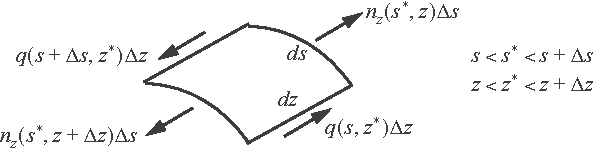
\includegraphics{Figure_3-10.pdf}}
\caption{Free body diagram for axial equilibrium of a differential element of the middle surface.}\label{fig3.10}
\end{figure}}

Summation of the forces in the $z$-direction yields
\begin{align}\label{eq3.85}
\left[n_{z}\left(s^{*}, z+\Delta z\right)-n_{z}\left(s^{*}, z\right)\right] \Delta s+\left[q\left(s+\Delta s, z^{*}\right)-q\left(s, z^{*}\right)\right] \Delta z=0.
\end{align}
Division by $\Delta s\Delta z$ followed by taking the limit as $\Delta s \rightarrow 0$ and $\Delta z \rightarrow 0$ yields the partial differential equation
\begin{align}\label{eq3.86}
\frac{\partial n_{z}}{\partial z}+\frac{\partial q}{\partial s}=0.
\end{align}
The normal stress resultant $n_z$ is given by eq.~(\ref{eq3.72}) and it is based on the kinematic assumption for the displacements made in article \ref{sec3.3}, infinitesimal deformation, and Hooke's law. The expression for the normal stress resultant is written as $n_{z}=t(s)[E \varepsilon_{z z}-\beta \Delta T]$. Substitute eq.~(\ref{eq3.82}) for the normal strain to get
\begin{align}\label{eq3.87}
n_{z}=t(s)\left[\frac{N+N_{T}}{A}+k \frac{\left(M_{x}+M_{x T}\right)}{I_{x x}} \bar{y}(s)+k \frac{\left(M_{y}+M_{y T}\right)}{I_{y y}} \bar{x}(s)-\beta \Delta T\right].
\end{align}
Take the partial derivative of the normal stress resultant (\ref{eq3.87}) with respect to $z$. In the process of taking the derivative we eliminate the derivative of the axial force using equilibrium eq.~(\ref{eq3.53}), and we eliminate the derivative of the bending moments using equilibrium eqs. (\ref{eq3.55}), and (\ref{eq3.57}). The final result for the derivative of the normal stress resultant with respect to $z$ is
\begin{align}\label{eq3.88}
\frac{\partial n_{z}}{\partial z}=\frac{t(s)}{A} \frac{d N_{T}}{d z}-\beta \frac{\partial \Delta T}{\partial z} t(s)+\frac{k}{I_{x x}}\left[V_{y}+V_{y T}\right] \bar{y}(s) t(s)+\frac{k}{I_{y y}}\left[V_{x}+V_{y T}\right] \bar{x}(s) t(s).
\end{align}
Assume differentiation with respect to $z$ can be interchanged with the definite integrals with respect to $s$ (Leibniz's rule). Then, the new terms in eq.~(\ref{eq3.88}) are given by the equations
\begin{align}\label{eq3.89}
\frac{d N_{T}}{d z}=\int_{c} \beta \frac{\partial \Delta T}{\partial z} t(s) d s \quad V_{x T}=\frac{d M_{y T}}{d z}=\int_{c} \beta \frac{\partial \Delta T}{\partial z} x(s) t(s) d s \quad V_{y T}=\frac{d M_{x T}}{d z}=\int_{c} \beta \frac{\partial \Delta T}{\partial z} y(s) t(s) d s.
\end{align}
The functions $V_{x T}(z)$ and $V_{y T}(z)$ are defined as thermal shear forces. Integrate the differential equation (\ref{eq3.86}) with respect to the contour coordinate from $s$ = 0 to $s$ = $s$ to get
\begin{align}\label{eq3.90}
\int_{0}^{s} \frac{\partial n_{z}}{\partial z}ds+q(s, z)-q(0, z)=0.
\end{align}
Solve the latter equation for the shear flow to write
\begin{align}\label{eq3.91}
q(s, z)=q_{0}(z)-\int_{0}^{s} \frac{\partial n_{z}}{\partial z} d s,
\end{align}
where $q_{0}(z)=q(0, z)$. Note that the origin of the contour coordinate where $s = 0$ is arbitrary at this point. Now the result for the integral with respect to the contour coordinate of the derivative of the normal stress resultant is written as
\begin{align}\label{eq3.92}
\int_{0}^{s} \frac{\partial n_{z}}{\partial z} d s=\frac{k}{I_{x x}} V_{y}(z) \bar{Q}_{x}(s)+\frac{k}{I_{y y}} V_{x}(z) \bar{Q}_{y}(s)+q_{T}(s, z).
\end{align}
In eq.~(\ref{eq3.92}) the functions $\bar{Q}_{x}    (s)$ and $\bar{Q}_{y}(s)$ are called distribution functions. They are defined with respect to coordinate functions $\bar{x}(s)$ and $\bar{y}(s)$ for the segment of the contour from $s = 0$ to $s$, and are given by
\begin{align}\label{eq3.93}
\bar{Q}_{x}(s)=\int_{0}^{s}[\bar{y}(s) t(s)] d s=Q_{x}(s)-n_{y} Q_{y}(s) \quad \bar{Q}_{y}(s)=\int_{0}^{s}[\bar{x}(s) t(s)] d s=Q_{y}(s)-n_{x} Q_{x}(s).
\end{align}
\clearpage

\noindent In eq.~(\ref{eq3.93}) the distribution functions with respect to the centroidal coordinates $x(s)$ and $y(s)$ are defined by
\begin{align}\label{eq3.94}
Q_{x}(s)=\int_{0}^{s} y(s) t(s) d s \quad Q_{y}(s)=\int_{0}^{s} x(s) t(s) d s.
\end{align}
The function $q_{T}(s, z)$ in eq.~(\ref{eq3.92}) is the shear flow from the temperature gradient in the axial coordinate $z$. It is defined by
\begin{align}
q_{T}(s, z)&=\frac{A(s)}{A} \int_{c} \beta \frac{\partial \Delta T}{\partial z} t(s) d s-\int_{0}^{s} \beta \frac{\partial \Delta T}{\partial z} t(s) d s+\frac{k}{I_{x x}}\left(\int_{c} \beta \frac{\partial \Delta T}{\partial z} y(s) t(s) d s\right) \bar{Q}_{x}(s)\nonumber\\
&\quad +\frac{k}{I_{y y}}\left(\int_{c} \beta \frac{\partial \Delta T}{\partial z} x(s) t(s) d s\right) \bar{Q}_{y}(s),\label{eq3.95}
\end{align}
where the area of the contour segment is
\begin{align}\label{eq3.96}
A(s)=\int_{0}^{s} t(s) d s.
\end{align}
The shear flow from the change in temperature vanishes for two practical cases: (1) The temperature is spatially uniform in the axial coordinate $z$ so that $\Delta T(s)$ and $\frac{\partial \Delta T}{\partial z}=0$, and (2) the change in temperature and material coefficient $\beta$ are spatially uniform over the cross section so $\Delta T=\Delta T(z)$.

Substitute the result for the integral in eq.~(\ref{eq3.92}) into eq.~(\ref{eq3.91}), we write the formula for the shear flow due to the transverse shear forces as
\begin{align}\label{eq3.97}
\fbox{$\displaystyle q(s, z)=q_{0}(z)-\frac{k}{I_{y y}} V_{x} \bar{Q}_{y}(s)-\frac{k}{I_{x x}} V_{y} \bar{Q}_{x}(s)-q_{T}(s, z)$}.
\end{align}

\subsection{ Open cross-sectional contour}\label{sec3.8.1}

From eq.~(\ref{eq3.97}) the shear flow at the contour origin is $q(0, z)=q_{0}(z)$. For most open cross sections, there is a longitudinal edge of the bar that is free of external tractions. If the contour origin is taken at the location of the free longitudinal edge, then $q(0, z)=q_{0}(z)=0$.The shear flow for an open cross section with the contour origin located at the longitudinal free edge and $q_{T}=0$ is given by
\begin{align}\label{eq3.98}
q(s, z)=-\frac{k}{I_{y y}} V_{x} \bar{Q}_{y}(s)-\frac{k}{I_{x x}} V_{y} \bar{Q}_{x}(s).
\end{align}

\vspace*{-1.4pc}

\begin{example}[Shear flow distribution in the open cross section shown in figure~\ref{fig3.1}]\label{ex3.2}\setcounter{equation}{0}\def\theequation{\alph{equation}}Take the change in temperature $\Delta T(s, z)=0$, $0 \leq s \leq S$, and $0 \leq z \leq L$. Hence, $q_{T}=0$ for the shear flow expression given by eq.~(\ref{eq3.98}). Second area moments were computed in example~\ref{ex3.1} page \pageref{ex3.1} with the results listed in eqs. (\textbf{l}) to (\textbf{n}). Cross-sectional properties that depend on the second area moments, eq.~(\ref{eq3.81}), are
\begin{align}\label{ex3.2a}
n_{x}=\frac{I_{x y}}{I_{x x}}=\frac{0.724359 a^{3} t}{3.36086 a^{3} t}=0.215528 \quad n_{y}=\frac{I_{x y}}{I_{y y}}=\frac{0.724359 a^{3} t}{0.604984 a^{3} t}=1.19732 \quad k=1.34781.
\end{align}

The first area moments of the segment of branch 1 from $s_{1}=0$ to $s_{1} \in[0, a]$ with respect the centroidal coordinates are
\begin{align}\label{ex3.2b}
Q_{x 1}=\int_{0}^{s_{1}} y_{1}\left(s_{1}\right) t d s_{1} \quad Q_{y 1}=\int_{0}^{s_{1}} x_{1}\left(s_{1}\right) t d s_{1}.
\end{align}
From eq. (\textbf{j}) of example~\ref{ex3.1} $x_{1}\left(s_{1}\right)=-0.482906 a$ and $y_{1}\left(s_{1}\right)=-1.63782 a+s_{1}$. Performing the integrals in the first area moments we get
\begin{align}\label{ex3.2c}
Q_{x 1}=\frac{t\left(-a-4 a \pi+s_{1}+\pi s_{1}\right) s_{1}}{2(1+\pi)}=-1.63782 a t s_{1}+0.50 t s_{1}^{2} \quad Q_{y 1}=\frac{-2 a t}{1+\pi} s_{1}=-0.482906 a t s_{1}.
\end{align}
The distribution functions of the segment with respect to the $\bar{x}$-$\bar{y}$ system are given by eq.~(\ref{eq3.93}), which for branch 1 results in
\begin{gather}
\bar{Q}_{x 1}=-1.63782 a t s_{1}+0.50 t s_{1}^{2}-(1.19732)\left(-0.482906 a t s_{1}\right)=-1.05963 a t s_{1}+0.5 t s_{1}^{2},\label{ex3.2d} \tag{d}\\
\bar{Q}_{y 1}=(-0.482906 a t s_{1})-(0.215528)(-1.63782 a t s_{1}+0.50 t s_{1}^{2})=-0.12991 a t s_{1}-0.107764 t s_{1}^{2}.\label{ex3.2e} \tag{e}
\end{gather}
At $s_1 = 0$, the longitudinal free edge condition requires $q_0 = 0$. The shear flow in branch 1 can now be computed from eq.~(\ref{eq3.98}). The result is
\begin{align}\label{ex3.2f}
q_{1}\left(s_{1}\right)=\left[0.289419\left(\frac{s_{1}}{a}\right)+0.240081\left(\frac{s_{1}}{a}\right)^{2}\right] \frac{V_{x}}{a}+\left[0.424944\left(\frac{s_{1}}{a}\right)-0.200516\left(\frac{s_{1}}{a}\right)^{2}\right] \frac{V_{y}}{a} \quad 0 \leq s_{1} \leq a. \tag{f}
\end{align}

\vspace*{-10pt}

The first area moments of the cross-sectional area consisting of branch 1 and a segment of branch 2 are given~by
\begin{align}\label{ex3.2g}
Q_{x 2}(\theta)=Q_{x 1}(a)+\int_{-\pi / 2}^{\theta} y_{2}(\theta) \textit{tad} \theta \quad Q_{y 2}(\theta)=Q_{y 1}(a)+\int_{-\pi / 2}^{\theta} x_{2}(\theta) \textit{tad} \theta. \tag{g}
\end{align}
where from eq. (\textbf{\ref{ex3.2c}}) we find
\begin{align}\label{ex3.2h}
Q_{x 1}(a)=(-1.13782) a^{2} t \quad Q_{y 1}(a)=(-0.482906) a^{2} t. \tag{h}
\end{align}
From eq. (\textbf{k}) of example~\ref{ex3.1} $x_{2}(\theta)=-0.482906 a+a \cos \theta$ and $y_{2}(\theta)=0.36218 a+a \sin \theta$. Evaluating the integrals in the first area moments for branch 2 we get
\begin{align*}
\int_{-\pi / 2}^{\theta} y_{2}(\theta) \textit{tad} \theta=(0.56891+0.36218 \theta-\cos \theta) a^{2} t \quad \int_{-\pi / 2}^{\theta} x_{2}(\theta) t a d \theta=(0.241453-0.482906 \theta+\sin \theta) a^{2} t.
\end{align*}
Thus, the first area moments of the cross-sectional area consisting of branch 1 and a segment of branch 2 are
\begin{gather}\label{ex3.2i}
\begin{split}
Q_{x 2}=((-1.13782)+0.56891+0.36218 \theta-\cos \theta) a^{2} t=(-0.56891+0.36218 \theta-\cos \theta) a^{2} t \\
Q_{y 2}=((-0.482906)+0.241453-0.482906 \theta+\sin \theta) a^{2} t=(-0.241453-0.482906 \theta+\sin \theta) a^{2} t.
\end{split}\tag{i}
\end{gather}
Note that at $\theta=\pi / 2$ both $Q_{x 2}=Q_{y 2}=0$, since the origin of the \textit{x-y} system is at centroid of the cross section (i.e., the first area moments of the entire cross-sectional area about the centroidal coordinate system vanish).

The first area moment $\bar{Q}_{x}$ given in eq.~(\ref{eq3.93}) for the cross-sectional area consisting of branch 1 plus a segment of branch 2 is computed as
\[
%\begin{align}
\bar{Q}_{x 2}=(-0.56891+0.36218 \theta-\cos \theta) a^{2} t-(1.19732)((-0.241453-0.482906 \theta+\sin \theta) a^{2} t).
%\end{align}
\]

\vspace*{-0.3pc}\pagebreak

\noindent Combining terms we get
\begin{align}\label{ex3.2j}
\bar{Q}_{x 2}=(-0.279814+0.940372 \theta-\cos \theta-1.19732 \sin \theta) a^{2} t.\tag{j}
\end{align}
The first area moment $\bar{Q}_{y}$ given in eq.~(\ref{eq3.93}) for the cross-sectional area consisting of branch 1 plus a segment of branch 2 is computed as
\begin{align}\label{ex3.2k}
\bar{Q}_{y 2}=(-0.241453-0.482906 \theta+\sin \theta) a^{2} t-(0.215528)((-0.56891+0.36218 \theta-\cos \theta) a^{2} t).\tag{k}
\end{align}
Combining terms we get
\begin{align}\label{ex3.2l}
\bar{Q}_{y_{2}}=(-0.118837-0.560966 \theta+0.215528 \cos \theta+\sin \theta) a^{2} t. \tag{l}
\end{align}
The shear flow in branch 2 can now be computed from eq.~(\ref{eq3.98}), which yields\vspace*{-4pt}
\begin{align}\label{ex3.2m}
q_{2}(\theta)=& [0.26475+1.24974 \theta-0.480162 \cos \theta-2.22784 \sin \theta] \frac{V_{x}}{a}\nonumber\\[-3pt]
& +[0.112214-0.377118 \theta+0.401031 \cos \theta+0.480162 \sin \theta] \frac{V_{y}}{a}. \tag{m}
\end{align}
Note that $q_{2}(\pi / 2)=0$, which is consistent with the vanishing of the shear flow at the top free edge. Shear flow distributions are plotted normal to the contour in figure~\ref{fig3.11}.
\end{example}

{\def\thefigure{3.11}
\processfigure{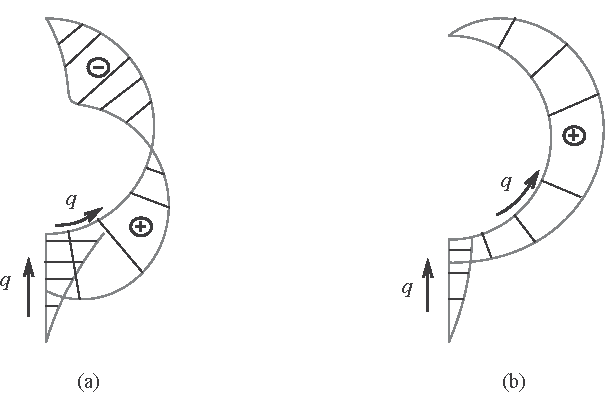
\includegraphics{Figure_3-11.pdf}}
{\caption{Shear flow distributions for the open section in figure~\ref{fig3.1}. (a) $V_x > \textbf{0}$ \& $V_y = \textbf{0}$. (b) $V_x = \textbf{0}$ \&\break $V_y > \textbf{0}$.}\label{fig3.11}}}


\setcounter{equation}{98}
\subsection{Location of the shear center for an open cross section}\label{sec3.8.2}

The shear flow given by eq.~(\ref{eq3.98}) is determined by transverse shear forces $V_x$ and $V_y$, and is independent of the torque $M_z$. For transverse bending the shear flow $q$ is the dominate term in the expression (\ref{eq3.40}) for the torque. Hence, the contribution of the twisting moment resultant $m_{zs}$ and the transverse stress resultant $q_z$ are neglected in eq.~(\ref{eq3.40}) with respect to the shear flow.\footnote{Note that $m_{zs}$ and $q_z$ are the main contributors to $M_z$ under pure torsion of an open section as is discussed in article \ref{sec3.9}.} The torque with respect to the shear center resulting from the shear flow is then
\begin{align}\label{eq3.99}
M_{z}=\int_{c} r_{n} q d s=\int_{c} r_{n}(s)\left[-\frac{k}{I_{y y}} V_{x} \bar{Q}_{y}(s)-\frac{k}{I_{x x}} V_{y} \bar{Q}_{x}(s)\right] d s.
\end{align}
Expanding eq.~(\ref{eq3.99}), we get
\begin{align}\label{eq3.100}
M_{z}=-\left[\left(\frac{k}{I_{y y}}\right) \int_{c} r_{n}(s) \bar{Q}_{y}(s) d s\right] V_{x}-\left[\left(\frac{k}{I_{x x}}\right) \int_{c} r_{n}(s) \bar{Q}_{x}(s) d s\right] V_{y}.
\end{align}
The contribution of the shear forces acting at the shear center to the torque in eq.~(\ref{eq3.100}) must vanish by the definition of the shear center. Thus,
\begin{align}\label{eq3.101}
-\left(\frac{k}{I_{y y}}\right)\left[\int_{c} r_{n}(s) \bar{Q}_{y}(s) d s \right] V_{x}-\left(\frac{k}{I_{x x}}\right)\left[\int_{c} r_{n}(s) \bar{Q}_{x}(s) d s \right] V_{y}=0 \quad \forall V_{x} \& V_{y}.
\end{align}
Equation (\ref{eq3.101}) can only be satisfied if
\begin{align}\label{eq3.102}
\int_{c} r_{n}(s) \bar{Q}_{y}(s) d s=0 \quad \int_{c} r_{n}(s) \bar{Q}_{x}(s) d s=0.
\end{align}

\vspace*{-1pc}

To locate the shear center relative to the centroid, substitute the expression for the normal coordinate $r_{n}(s)$ from eq.~(\ref{eq3.10}) into the preceding geometric properties of the shear center to get
\begin{gather}
\int_{c} r_{n}(s) \bar{Q}_{y}(s) d s=\int_{c} r_{n c}(s) \bar{Q}_{y}(s) d s-x_{s c} \int_{c} \bar{Q}_{y}(s) \frac{d y}{d s} d s+y_{s c} \int_{c} \bar{Q}_{y}(s) \frac{d x}{d s} d s=0\mbox{, and}\label{eq3.103}\\
\int_{c} r_{n}(s) \bar{Q}_{x}(s) d s=\int_{c} r_{n c}(s) \bar{Q}_{x}(s) d s-x_{s c} \int_{c} \bar{Q}_{x}(s) \frac{d y}{d s} d s+y_{s c} \int_{c} \bar{Q}_{x}(s) \frac{d x}{d s} d s=0.\label{eq3.104}
\end{gather}
With the aid of eqs. (\ref{eq3.93}), (\ref{eq3.84}), (\ref{eq3.81}), and (\ref{eq3.77}), integrate by parts the following terms in eqs. (\ref{eq3.103}) and (\ref{eq3.104}) to find
\begin{align}\label{eq3.105}
\int_{c} \bar{Q}_{y}(s)\left(\frac{d x}{d s}\right) d s=\frac{-I_{y y}}{k} \quad \int_{c} \bar{Q}_{x}(s)\left(\frac{d x}{d s}\right) d s=0 \quad \int_{c} \bar{Q}_{y}(s)\left(\frac{d y}{d s}\right) d s=0 \quad \int_{c} \bar{Q}_{x}(s)\left(\frac{d y}{d s}\right) d s=\frac{-I_{x x}}{k}.
\end{align}
Substitute the results from eq.~(\ref{eq3.105}) into eqs. (\ref{eq3.103}) and (\ref{eq3.104}), and then solve for the coordinates of the shear center relative to the centroid as
\begin{align}\label{eq3.106}
\fbox{$\displaystyle x_{s c}=-\left(\frac{k}{I_{x x}}\right)\left[\int_{c} r_{n c}(s) \bar{Q}_{x}(s) d s\right] \quad y_{s c}=\frac{k}{I_{y y}}\left[\int_{c} r_{n c}(s) \bar{Q}_{y(s)} d s\right]$}.
\end{align}
Note that normal coordinate $r_{n c}(s)$ is computed from the second of eq.~(\ref{eq3.11}) once the contour coordinates with respect to the centroid are established.\vspace*{-10pt}

\begin{example}[Shear center of the open section shown in figure~\ref{fig3.1}]\label{ex3.3}\setcounter{equation}{0}\def\theequation{\alph{equation}}\textbf{Method 1.}{\quad}For the open section consisting of two branches, the coordinates of the shear center relative to the centroid from eq.~(\ref{eq3.106}) are given by
\begin{align*}
x_{s c}=\left(-k / I_{x x}\right)\left(\int_{0}^{a} r_{n c 1} \bar{Q}_{x 1} d s_{1}+\int_{-\pi / 2}^{\pi / 2} r_{n c 2} \bar{Q}_{x 2} a d \theta\right) \quad y_{s c}=\left(k / I_{y y}\right)\left(\int_{0}^{a} r_{n c 1} \bar{Q}_{y 1} d s_{1}+\int_{-\pi / 2}^{\pi / 2} r_{n c 2} \bar{Q}_{y 2} a d \theta\right).
\end{align*}
\vspace*{2pt}
\clearpage

\noindent Some of the terms in these formulas are listed as eqs. (\textbf{\ref{ex3.1l}}) and (\textbf{\ref{ex3.1m}}) in example~\ref{ex3.1} page \pageref{ex3.1}, and eqs. (\textbf{\ref{ex3.2d}}), (\textbf{\ref{ex3.2c}}), (\textbf{j})), and (\textbf{l}) in example~\ref{ex3.2} on page \pageref{ex3.2d}. We list these terms for convenience as follows:
\begin{gather*}
k=1.34781 \quad I_{x x}=3.36086 a^{3} t \quad I_{y y}=0.604984 a^{3} t,\\
\bar{Q}_{x 1}=-1.05963 a t s_{1}+0.5 t s_{1}^{2} \quad \bar{Q}_{y 1}=-0.12991 a t s_{1}-0.107764 t s_{1}^{2}\mbox{, and}\\
\bar{Q}_{x 2}=(-0.279814+0.940372 \theta-\cos \theta-1.19732 \sin \theta) a^{2} t \\
\bar{Q}_{y 2}=(-0.118837-0.560966 \theta+0.215528 \cos \theta+\sin \theta) a^{2} t.
\end{gather*}
From eq.~(\ref{eq3.11}) the coordinates normal to the contour relative to the centroid are given by
\begin{align*}
r_{n c 1}=x_{1}\left(\frac{d y_{1}}{d s_{1}}\right)-y_{1}\left(\frac{d x_{1}}{d s_{1}}\right) \quad r_{n c 2}=\frac{x_{2}}{a}\left(\frac{d y_{2}}{d \theta}\right)-\frac{y_{2}}{a}\left(\frac{d x_{2}}{d \theta}\right).
\end{align*}
The Cartesian coordinates of the contour for each branch are given by eqs.~(\textbf{\ref{ex3.1j}}) and (\textbf{\ref{ex3.1k}}) in example~\ref{ex3.1}, which are repeated below:
\begin{gather*}
\begin{array}{lll}
x_{1}\left(s_{1}\right)=-0.482906 a & y_{1}\left(s_{1}\right) =-1.63782 a+s_{1} & 0 \leq s_{1} \leq a \\
x_{2}(\theta)=-0.482906 a+a \cos \theta & y_{2}(\theta) =0.36218 a+a \sin \theta & -\pi / 2 \leq \theta \leq \pi / 2\end{array}.
\end{gather*}
The results for the coordinates normal to the contour are
\begin{align*}
r_{n c 1}=-0.482906 a \quad r_{n c 2}=a(1-0.482906 \cos \theta+0.36218 \sin \theta).
\end{align*}
The shear center coordinates are determined from the following integrals
\begin{align*}
x_{s c}=&\left(\frac{-1.34781}{3.36086 a^{3} t}\right)\left[\int_{0}^{a}(-0.482906 a)(-1.05963 a t s_{1}+0.5 t s_{1}^{2}) d s_{1}\right. \\
&+\!\!\left.\int_{-\pi / 2}^{\pi / 2}[a(1-0.482906 \cos \theta+0.36218 \sin \theta)]\left[(-0.279814+0.940372 \theta-\cos \theta-1.19732 \sin \theta) a^{2} t\right] a d \theta\right]\\
y_{s c}=&\left(\frac{1.34781}{0.604984 a^{3} t}\right)\left[\int_{0}^{a}(-0.482906 a)(-0.12991 a t s_{1}-0.107764 t s_{1}^{2}) d s_{1}\right.\\
&+\!\!\left.\int_{-\pi / 2}^{\pi / 2}\![a(1-0.482906 \cos \theta+0.36218 \sin \theta)]\!  \left[(-0.118837-0.560966 \theta+0.215528 \cos \theta+\sin \theta) a^{2} t\right] a d \theta\right]\!.
\end{align*}
The preceding integrals were evaluated in \textit{Mathematica} to get
\begin{align}\label{ex3.3a}
x_{s c}=0.67169 a \quad y_{s c}=0.490767 a. \tag{a}
\end{align}

\vspace*{-1pc}

\noindent\textbf{Method 2.}{\enspace}The shear flow distributions were determined in example \ref{ex3.2} on page \pageref{ex3.2} with the results given by eq. (\textbf{f}) for branch 1 and by eq. (\textbf{m}) for branch 2. These shear flows are illustrated in the left-hand sketch in figure~\ref{fig3.12}. It is convenient to determine the resultant of the shear flow distribution at point $O$ first. As shown in figure~\ref{fig3.12} the components of the resultant force are $F_{X}$ and $F_{Y}$, and the torque is $M_{z 0}$. Under transverse bending the contributions of the transverse shear resultant $q_{z}$ and twisting moment resultant $m_{z s}$ are negligible with respect to the shear flow \textit{q} in the expressions for the shear forces and the torque\footnote{Under pure torsion the transverse shear resultant and the twisting moment resultant are the major contributors to the torque as discussed in article~3.9.} in eq.~(\ref{eq3.40}). Hence, the force components and the torque are given by the following integrals of the shear flow over the contour.\pagebreak
\begin{align}\label{ex3.3b}
F_{X}=\int_{-\pi / 2}^{\pi / 2} q_{2}(\theta)(-\sin \theta) a d \theta \quad F_{Y}=\int_{0}^{a} q_{1}\left(s_{1}\right) d s_{1}+\int_{-\pi / 2}^{\pi / 2} q_{2}(\theta)(\cos \theta) a d \theta \quad M_{z_{0}}=\int_{-\pi / 2}^{\pi / 2} a\left[q_{2}(\theta) a d \theta\right]. \tag{b}
\end{align}
The line of action of the shear flow in branch 1 is parallel to the $Y$-direction and so does not contribute to the force component $F_{X}$ in eq. (\textbf{\ref{ex3.3b}}). From example~\ref{ex3.2} substitute eq. (\textbf{\ref{ex3.2d}}) for $q_{1}$ and eq.~(\textbf{\ref{ex3.2h}}) for $q_{2}$ into eq. (\textbf{\ref{ex3.3b}}) above, then perform the integrations, to find $F_{X}=V_{x}$ and $F_{Y}=V_{y}$. It is expected that the force components would be equal to their respective transverse shear components, since the shear flows were determined from equilibrium conditions with respect to the transverse shear forces in article \ref{sec3.8}. Only the shear flow in branch 2 contributes to the torque about point $O$, since the line of action of the shear flow in branch 1 passes through point $O$. The moment arm to the differential force $q_{2} a d \theta$ in branch 2 about point $O$ is simply the radius $a$. From example~\ref{ex3.2} substitute eq. (\textbf{\ref{ex3.2h}}) for $q_{2}$ in the expression for the torque in eq. (\textbf{\ref{ex3.3b}}) above, and perform the integration to get
\begin{align}\label{ex3.3c}
M_{z 0}=-0.128587 a V_{x}+1.15459 a V_{y}. \tag{c}
\end{align}
{\def\thefigure{3.12}
\def\floataboveskip{-15pt}
\processfigure[H]{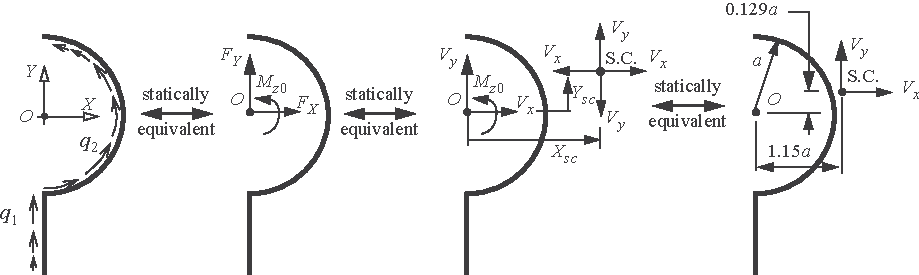
\includegraphics{Figure_3-12.pdf}
}{\caption{Resultant of the shear flow distribution.\label{fig3.12}\vspace*{-12pt}}}}
Now add and subtract the shear forces $V_x$ and $V_y$ at the shear center (S.C.) in order to preserve force equivalence as is shown in figure~\ref{fig3.12}. The upward force $V_y$ at point $O$ and the downward force $V_y$ at S.C. form a clockwise couple $X_{s c} V_{y}$ and no net vertical force. Similarly, force $V_x$ at point $O$ and the equal and opposite force $V_x$ at the S.C. form a counterclockwise couple $Y_{s c} V_{x}$ and no net horizontal force. The total counterclockwise torque in the cross section must vanish by the definition of the S.C.; i.e., $M_{z 0}-X_{s c} V_{y}+Y_{s c} V_{x}=0$. Substitute eq.~(\textbf{\ref{ex3.3c}}) for $M_{z 0}$ in the total torque to get
\begin{align}\label{ex3.3d}
\left(-0.128587 a+Y_{s c}\right) V_{x}+\left(1.15459 a-X_{s c}\right) V_{y}=0 \quad \forall\left(V_{x}, V_{y}\right). \tag{d}
\end{align}
Therefore, the location of the shear center relative to point $O$ is given by
\begin{align}\label{ex3.3e}
X_{s c}=1.15459 a \quad Y_{s c}=0.128587 a. \tag{e}
\end{align}
The coordinates of the shear center relative to the centroid are given by $x_{s c}=X_{s c}-X_{c}$ and $y_{s c}=Y_{s c}-Y_{c}$, where the coordinates of the centroid relative to point $O$ is given by eq. (\textbf{\ref{ex3.1i}}) in example~\ref{ex3.1} on page \pageref{ex3.1}. Thus,
\begin{align}\label{ex3.3f}
x_{s c}=1.15459 a-0.48290 a=0.67169 a \quad y_{s c}=0.128587 a-(-0.36218 a)=0.490767 a, \tag{f}
\end{align}
which is the same result obtained in eq. (\textbf{\ref{ex3.3a}}) by method 1.
\end{example}

\subsection{Notes concerning the shear center}\label{sec3.8.3}

\begin{itemize}
\item The resultant of the shear flow distribution over the contour is a force with components $V_x$ and $V_y$ acting through the shear center such that there is no torque acting at the shear center. If the cross section is subject to a torque, this torque cannot be balanced by the shear flow which, according to eq.~(\ref{eq3.98}), is uniquely determined by the shear forces $V_x$ and $V_y$.

\item The location of the shear center in the cross section is determined by the pattern of the shear flow distribution and not on the magnitude of the transverse shear forces.

\item Transverse shear forces $V_x$ and $V_y$ act in the plane of loading to equilibrate the externally applied lateral load intensities $f_{x}(z)$ and $f_{y}(z)$. (Refer to equilibrium equations (\ref{eq3.54}) and (\ref{eq3.56}).) Thus, the line of action of the external lateral loads must pass through the shear center to bend the bar without twisting it in torsion.

\item The shear center is located on an axis of symmetry of the cross section if there is one. If there are two axes of symmetry in the cross section the shear center and the centroid lie on the intersection of the symmetry axes.

\item For an open cross section with straight branches and one junction the shear center is at the junction, since the torque from the shear flows at the junction vanishes. See figure~\ref{fig3.13}.
\end{itemize}

{\def\thefigure{3.13}
\begin{figure}[!h]
\centerline{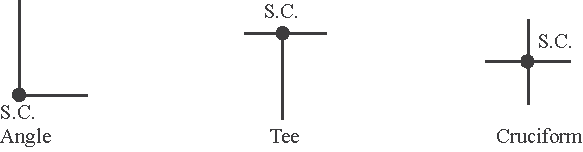
\includegraphics{Figure_3-13.pdf}}
\caption{Shear center locations for open sections with straight branches and one junction.}\label{fig3.13}
\end{figure}}

\vspace*{-1pc}
\setcounter{equation}{106}
\section{Torsion of an open section with a straight contour}\label{sec3.9}

Although we have located the shear center for the open cross-sectional contour, a material law for the torque acting at the shear center remains to be determined. Torsion of an open section bar is an important problem in engineering, but it is not a simple problem in elasticity. Saint-Venant (1855) guided by the solution of the bar with a circular cross section, made a brilliant guess and showed that an exact solution to a well-defined problem can be obtained. Here, we consider a simplified approach following the presentation given by Vasiliev (1993).

Consider a prismatic bar with a rectangular cross section subject to equal and opposite torques acting on the end cross sections at $z=0$ and $z=L$. The lateral surfaces of the bar are traction free so $p_n = p_s = p_z =0$ in eqs.~(\ref{eq3.42}) and $m_z (z) = 0$ in  (\ref{eq3.45}) on page \pageref{eq3.44} for $0 \leq z \leq L$. Equilibrium equations (\ref{eq3.53}) to (\ref{eq3.57}) are identically satisfied when $N=V_{x}=V_{y}=M_{x}=M_{y}=0$ for $0 \leq z \leq L$, and torsional equilibrium (\ref{eq3.58}) is satisfied for a torque $M_{z}$ independent of axial coordinate $z$. Also, there is no change in temperature from the reference state $\Delta T=0$. For a Hookean material the twist per unit length $d \phi_{z} / d z$ is proportional to the torque, and so it is also a constant with respect to the $z$-coordinate.


The contour of a rectangular cross section is a straight horizontal line of length $b$ as shown in figure~\ref{fig3.14}. The angle $\theta=90^{\circ}$ in figure~\ref{fig3.3} for all values of $s$, and the geometric relations given by eqs. (\ref{eq3.3}) to (\ref{eq3.6}) and (\ref{eq3.8}) specialize to
\begin{align*}
x=-s \quad y=0 \quad \hat{t}=-\hat{i} \quad \hat{n}=\hat{j} \quad r_{t}=s \quad r_{n}=0 \quad d \theta / d s=1 / R_{s}=0.
\end{align*}
The cross-sectional coordinates are $(s, \zeta)$ with $s \in[-b / 2,\; b / 2]$ and $\zeta \in[-t / 2,\; t / 2]$, and the origin is the location of the centroid and also of the shear center.

{\def\thefigure{3.14}
\begin{figure}[!t]
\centerline{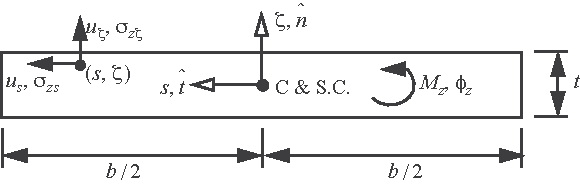
\includegraphics{Figure_3-14.pdf}}
\caption{A bar with rectangular cross section subject to uniform torsion.}\label{fig3.14}
\end{figure}}


\subsubsection{Displacements and strains.} Saint-Venant assumed that as the bar twists the cross section is displaced normal to the $s$-$\zeta$ plane (i.e., it warps) but its projection on the $s$-$\zeta$ plane rotates as a rigid body. To prevent rigid body displacement, the displacement components of the centroid are set equal to zero. Then, the in-plane displacements given by eqs. (\ref{eq3.20}) and (\ref{eq3.22}) reduce to
\begin{align}\label{eq3.107}
u_{\zeta}(s, z, \zeta)=-s \phi_{z}(z) \quad u_{s}(s, z, \zeta)=\zeta \phi_{z}(z).
\end{align}
The out-of-plane displacement given by eq.~(\ref{eq3.26}) is
\begin{align}\label{eq3.108}
u_{z}(s, z, \zeta)=-s \phi_{y}(z)+\zeta\left[\phi_{x}(z)\right].
\end{align}
However, this out-of-plane displacement is changed to account for the warping of the cross section in uniform torsion. \textbf{It is assumed that the rotation about the $\textbf{\textit{x}}$-axis, or the negative $\textbf{\textit{s}}$-axis, is independent of the $\textbf{\textit{z}}$-coordinate but is an unknown function of the $\textbf{\textit{s}}$-coordinate}. Consequently, the out-of-plane displacement in eq.~(\ref{eq3.108}) is changed to
\begin{align}\label{eq3.109}
u_{z}(s, z, \zeta)=\zeta \phi_{x}(s)-s \phi_{y}(z).
\end{align}

\vspace*{-1pc}

The only non-zero strains determined from the displacements (\ref{eq3.107}) and (\ref{eq3.109}) are shear strains $\gamma_{z s}$ and $\gamma_{z \zeta}$, From the strain-displacement relations given by eq.~(\ref{eq3.28}) these shear strain-displacement relations are
\begin{align}\label{eq3.110}
\gamma_{z s}=\left(\frac{d \phi_{z}}{d z}+\frac{d \phi_{x}}{d s}\right) \zeta-\phi_{y} \quad \gamma_{z \zeta}=\phi_{x}-s \frac{d \phi_{z}}{d z}.
\end{align}
Hooke's laws for the shear stresses are $\sigma_{z s}=G \gamma_{z s}$ and $\sigma_{z \zeta}=G \gamma_{z \zeta}$.

\subsubsection{Stress resultants and equilibrium.} The stress resultants associated with these non-zero shear strains (\ref{eq3.110}) are determined from Hooke's law, and the definition of stress resultants $q$, $m_{z s}$, and $q_{z}$ in eq.~(\ref{eq3.37}). The expressions for the stress resultants are
\begin{align}\label{eq3.111}
&\left(q, m_{z s}\right)=\hspace*{-3pt}\int_{-t / 2}^{t / 2}(1, \zeta) \sigma_{z s} d \zeta=G\hspace*{-3pt} \int_{-t / 2}^{t / 2}(1, \zeta)\left[\left(\frac{d \phi_{z}}{d z}+\frac{d \phi_{x}}{d s}\right) \zeta-\phi_{y}\right] d \zeta \nonumber\\ &q_{z}=\int_{-t / 2}^{t / 2}\hspace*{-4pt} \sigma_{z \zeta} d \zeta=G \int_{-t / 2}^{t / 2}\left(\phi_{x}-s \frac{d \phi_{z}}{d z}\right) d \zeta.
\end{align}
Performing the integrations through the thickness in eq.~(\ref{eq3.111}) we find the stress resultants are given by
\begin{align}\label{eq3.112}
q=-G t \phi_{y} \quad m_{z s}=\frac{G t^{3}}{12}\left(\frac{d \phi_{z}}{d z}+\frac{d \phi_{x}}{d s}\right) \quad q_{z}=G t\left(\phi_{x}-s \frac{d \phi_{z}}{d z}\right).
\end{align}

\vspace*{-1pc}

Since $V_{x}=V_{y}=q_{T}=0$, the shear flow from eq.~(\ref{eq3.97}) reduces to $q(s, z)=q_{0}(z)$. That is, the shear flow is spatially uniform in the $s$-coordinate. Furthermore, the longitudinal edges at $s=\pm b / 2$ are free of tractions, which means the shear flow vanishes. Hence, $q=0$ for $-b / 2 \leq s \leq b / 2$. It follows from the first equation in (\ref{eq3.112}) that rotation $\phi_{y}=0$.

\begin{wrapfigure}[12]{R}{196pt}\vspace*{-15pt}
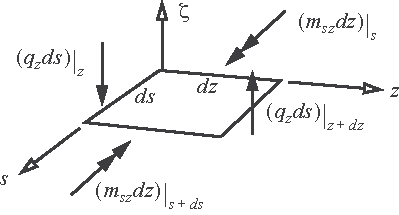
\includegraphics{Figure_3-15.pdf}
\caption{FBD for moments about the $s$-axis.\label{fig3.15}}
\end{wrapfigure}


The twisting moment resultant $m_{s z}$ and the transverse shear resultant $q_{z}$ are related by moment equilibrium about the $s$-axis for a differential element \textit{ds} by \textit{dz} cut from the wall. From the free body diagram for differential element of the wall shown in figure~\ref{fig3.15} moment equilibrium gives
\begin{align}
&\left.\frac{d z}{2}\left(q_{z} d s\right)\right|_{z+d z}\!\!+\left.\frac{d z}{2}\left(q_{z} d s\right)\right|_{z}\!-[\left.(m_{s z} d z)\right|_{s+d s}-\left.(m_{s z} d z)\right|_{s}] \nonumber\\
&\quad =0. \label{eq3.113}
\end{align}
Division of eq.~(\ref{eq3.113}) by area element \textit{ds} by \textit{dz}, followed by the limit as $d s \rightarrow 0$ and $d z \rightarrow 0$ yields the moment equilibrium differential\vspace*{-8pt} equation
\begin{align}\label{eq3.114}
q_{z}-\frac{d m_{s z}}{d s}=0.
\end{align}

\vspace*{-12pt}

\subsubsection{Governing boundary value problem.} Substitute $m_{z s}$ from eq.~(\ref{eq3.112}) into the differential equation (\ref{eq3.114}), followed by substitution of $q_{z}$ from eq.~(\ref{eq3.112}) into (\ref{eq3.114}). After these substitutions and re-arrangement, the result\vspace*{-5pt} is
\begin{align}\label{eq3.115}
\frac{d^{2} \phi_{x}}{d s^{2}}-\frac{12}{t^{2}} \phi_{x}=-\left(\frac{12}{t^{2}} \frac{d \phi_{z}}{d z}\right) s \quad \phi_{x}=\phi_{x}(s) \quad-b / 2<s<b / 2.
\end{align}
The longitudinal edges at $s=\pm b / 2$ are free of tractions, which additionally means the twisting moment $m_{s z}$ vanishes at $s=\pm b / 2$. From eq.~(\ref{eq3.112}) the vanishing of the twisting moment at the end points leads to the boundary condition\vspace*{-4pt}s
\begin{align}\label{eq3.116}
\frac{d \phi_{z}}{d z}+\frac{d \phi_{x}}{d s}=0 \quad~\text{at } s=\pm b / 2.
\end{align}
The solution to differential equation (\ref{eq3.115}) subject to boundary conditions (\ref{eq3.116})\vspace*{-4pt} is
\begin{align}\label{eq3.117}
\phi_{x}(s)=\left[s-\frac{2}{k} \frac{\sinh k s}{\cosh \lambda}\right] \frac{d \phi_{z}}{d z},
\end{align}
\vspace*{-20pt}
\removelastskip

\noindent wher\vspace*{-10pt}e
\begin{align}\label{eq3.118}
k=\frac{2 \sqrt{3}}{t} \quad \lambda=\frac{k b}{2}=\sqrt{3}\left(\frac{b}{t}\right).
\end{align}

\removelastskip

Substitute the solution for $\phi_{x}(s)$ from (\ref{eq3.117}) into the expressions for the twisting moment $m_{z s}$ and transverse shear $q_{z}$ listed in (\ref{eq3.112}) to\vspace*{-4pt} find
\begin{align}\label{eq3.119}
m_{z s}=\frac{G t^{3}}{6}\left(1-\frac{\cosh k s}{\cosh \lambda}\right)\left(\frac{d \phi_{z}}{d z}\right) \quad q_{z}=-2 G t \frac{\sinh k s}{k \cosh \lambda}\left(\frac{d \phi_{z}}{d z}\right).
\end{align}

\removelastskip

From the third expression in eq.~(\ref{eq3.40}) the torque about the $z$-axis, counterclockwise positive, is given\vspace*{-4pt} by
\begin{align}\label{eq3.120}
M_{z}=\int_{-b / 2}^{b / 2}\left(m_{z s}-s q_{z}\right) d s.
\end{align}
Substituting the results for $m_{z s}$ and $q_{z}$ from eq.~(\ref{eq3.119}) into the expression for the torque we write the result as
\begin{align}\label{eq3.121}
M_{z}=G J\left(\frac{d \phi_{z}}{d z}\right),
\end{align}
where the torsion constant $J$ is given by the integral
\begin{align*}
J=\int_{-b / 2}^{b / 2}\left[\frac{t^{3}}{6}\left(1-\frac{\cosh (k s)}{\cosh \lambda}\right)+2 t s\left(\frac{\sinh (k s)}{k \cosh \lambda}\right)\right] d s.
\end{align*}
After performing the integration, the result for the torsion constant is
\begin{align}\label{eq3.122}
J=\frac{b t^{3}}{3}\left(1-\frac{\tanh \lambda}{\lambda}\right).
\end{align}
For a thin, elongated rectangular cross section the value of the ratio of $b / t \gg 1$, which from the expression for $\lambda$ in eq.~(\ref{eq3.118}) implies $\lambda \gg 1$. In the limiting case of $\lambda \rightarrow \infty$ we find
\begin{align}\label{eq3.123}
J=\frac{b t^{3}}{3} \quad~\text{as } \quad \lambda \rightarrow \infty.
\end{align}
In the simplified theory of thin-walled open section bars, the torsion constant in each open branch is given by eq.~(\ref{eq3.123}).



The distribution of the twisting moment resultant $m_{z s}$ over the length of the contour for $b/t = 20$ is shown in figure~\ref{fig3.16}. As shown in the plot the distribution of $m_{z s}$ is symmetric with respect to the contour coordinate, attains a uniform magnitude over the majority of the contour, and decreases rapidly to zero near the boundaries of the contour where $s=\pm b / 2$. The distribution of the transverse shear resultant $q_{z}$ over the contour is shown in figure~\ref{fig3.17}. The distribution of $q_{z}$ is antisymmetric with respect to the contour coordinate, it is essentially equal to zero over the majority of the contour, and its maximum magnitude occurs in the narrow boundaries of the contour at $s=\pm b / 2$.

{\def\thefigure{3.16}
\begin{figure}[!b]
\centering{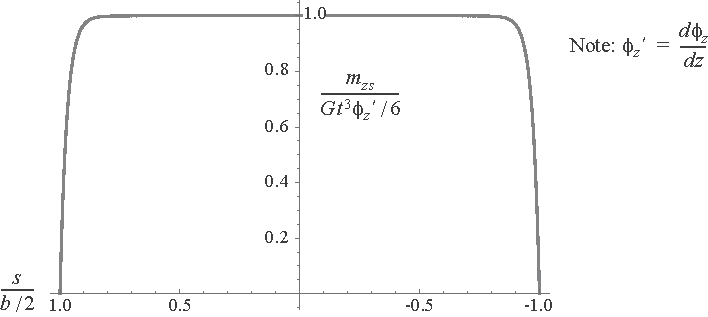
\includegraphics{Figure_3-16.pdf}}
\caption{Distribution of the twisting moment resultant over the contour for $b/t = \textbf{20}$.}\label{fig3.16}
\end{figure}}

{\def\thefigure{3.17}
\processfigure[H]{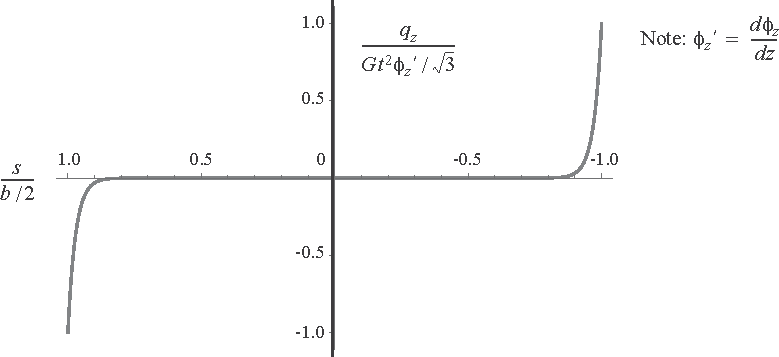
\includegraphics{Figure_3-17.pdf}
}{\caption{Distribution of the shear stress resultant over the contour for $b/t = \textbf{20}$.\label{fig3.17}}}}

From Hooke's law and eq.~(\ref{eq3.110}), the shear stress component tangent to the contour is
\begin{align*}
\sigma_{z s}=G \gamma_{z s}=G\left(\frac{d \phi_{z}}{d z}+\frac{d \phi_{x}}{d s}\right) \zeta.
\end{align*}
Substitute the solution for $\phi_{x}$ from eq.~(\ref{eq3.117}) into the previous equation to get
\begin{align}\label{eq3.124}
\sigma_{z s}(s, \zeta)=2 G\left(\frac{d \phi_{z}}{d z}\right)\left(1-\frac{\cosh (k s)}{\cosh \lambda}\right) \zeta.
\end{align}
Note that this shear stress vanishes on the contour where $\zeta=0$ and attains its maximum magnitude along the top and bottom edges where $\zeta=\pm t / 2$. Shear stress $\sigma_{Z s}$ is the dominate shear stress in the rectangular cross section subject to uniform torsion, since through-the-thickness shear stress $\sigma_{z \zeta}=q_{z} / t$ is essentially zero over most of the contour. For large values of $b/t$, we neglect the shear stress $\sigma_{z \zeta}$ with respect to $\sigma_{z s}$, and we use the following approximation
\begin{align}\label{eq3.125}
\sigma_{z s}=2 G\left(\frac{d \phi_{z}}{d z}\right) \zeta \quad b / t \gg 1.
\end{align}

\vspace*{-1pc}

\subsubsection{Warping of the cross section.} Substitute eq.~(\ref{eq3.117}) for $\phi_{x}(s)$ in eq.~(\ref{eq3.109}), and recall that $\phi_{y}=0$, to find that the warping displacement $u_{z}(s, \zeta)$ is given by
\begin{align}\label{eq3.126}
u_{z}(s, \zeta)=\zeta\left[s-\frac{t}{\sqrt{3}} \frac{\sinh k s}{\cosh \lambda}\right]\left(\frac{d \phi_{z}}{d z}\right).
\end{align}
\noindent A contour plot of the warping displacement divided by $u_{z}(b / 2, t / 2)$ for $b / t=4$ and $\frac{d \phi_{z}}{d z}>0$ is shown in figure~\ref{fig3.18}, where
\begin{align*}
u_{z}(b / 2, t / 2)=0.7113 t^{2}\left(\frac{d \phi_{z}}{d z}\right) \quad b / t=4.
\end{align*}
\noindent Along the $s$-axis and the $\zeta$-axis the warping displacement is zero, and it attains maximum magnitude near the corners of the rectangular cross section. For a positive unit twist, $u_{z}>0$ if the product $s \zeta>0$, and $u_{z}<0$ if the product $s \zeta<0$.

{\def\thefigure{3.18}
\processfigure[H]{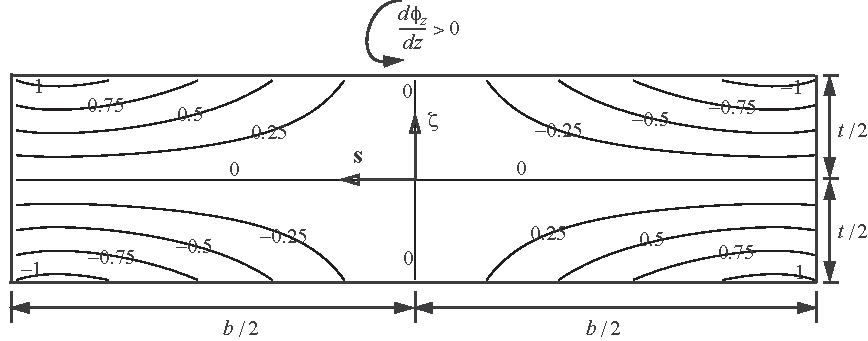
\includegraphics{Figure_3-18.pdf}
}{\caption{Contour plot of the normalized warping displacement in torsion for $b/t = \textbf{4}$.\label{fig3.18}}}}

For a thin rectangular cross section a good approximation to the warping function is
\begin{align}\label{eq3.127}
u_{z} \approx u_{z a}=s \zeta \quad b / t \gg 1.
\end{align}
To show eq.~(\ref{eq3.127}) is a good approximation, let
\begin{align*}
I_{e}=\left(\int_{-t / 2}^{t/2}\int_{-b / 2}^{b/2}\left[u_{z}(s, \zeta)\right]^{2} d s d \zeta\right)^{1 / 2}\mbox{ and }
I_{a}=\left(\int_{-t / 2}^{t/2}\int_{-b / 2}^{b/2}\left[u_{z a}(s, \zeta)\right]^{2} d s d \zeta\right)^{1 / 2}.
\end{align*}
Define the percentage error between the approximate warping function and the exact one by $\textrm{error} = (I_{a}-I_{e})\break 100 / I_{e}$. For $b / t=20$ the error is 0.482 percent, and for $b / t=40$ the error is 0.123 percent.

\subsection{Torsion of built-up open sections}\label{sec3.9.1}

For large values of the ratio of \textit{b/t}, the analysis of thin-walled rectangular section of article \ref{sec3.9} results in the following formulas given by eqs (\ref{eq3.121}), (\ref{eq3.123}), and (\ref{eq3.125}):
\begin{align}\label{eq3.128}
M_{z}=G J\left(\frac{d \phi_{z}}{d z}\right) \quad J=\frac{b t^{3}}{3} \quad \sigma_{z s}=2 G\left(\frac{d \phi_{z}}{d z}\right) \zeta.
\end{align}
The maximum magnitude of the shear stress $\sigma_{z s}$ occurs at $\zeta=\pm t / 2$. Then from the previous equations for large values of the ratio of \textit{b/t} this maximum shear stress can be expressed as
\begin{align}\label{eq3.129}
\left.\sigma_{z s}\right|_{\max }=\frac{3 M_{z}}{b t^{2}}.
\end{align}

\vspace*{-1pc}


Now consider torsion of open section bars of more complex shape as are shown in figure~\ref{fig3.19}. Understanding the torsional response of these bars with complex, open cross-sectional shapes is facilitated by an analogy to\vadjust{\pagebreak} the response of an initially flat membrane supported on its edges over an opening, where the edges of the opening are in the same shape as the cross section. The membrane is stretched under a uniform tension, and then subject to an internal pressure to cause the membrane to deflect. The deflected shape of this pressurized membrane is analogous to the torsion problem in that level contours on the surface of the deflected membrane coincide with the lines of action of the shear stresses, and that the slope of the membrane normal to the level contour is proportional to the magnitude to the shear stress. Also, the volume between the \textit{x-y} plane and the deflected surface of the membrane is proportional to the total torque carried by the section. The following text excerpted from Oden and Ripperger (1981, p.~46) summarizes this analogy.

%\vspace*{-12pt}

{\def\thefigure{3.19}
\processfigure[t]{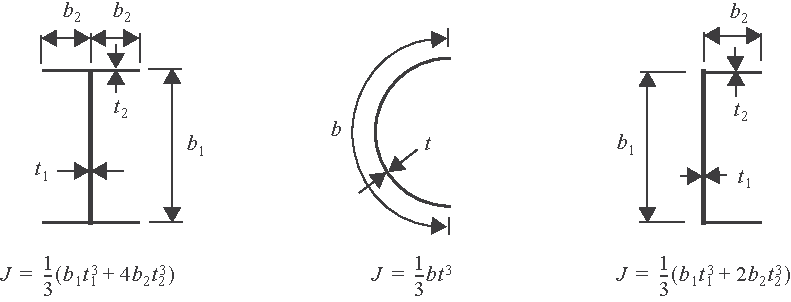
\includegraphics{Figure_3-19.pdf}
}{\caption{Some thin-walled open sections and their torsion constants.\label{fig3.19}}}}

\begin{quote}
\textit{This analogy was first discovered by Ludwig Prandtl in 1903 and is known as \textbf{Prandtl's membrane analogy.} Prandtl took full advantage of the analogy and devised clever experiments with membranes. By measuring the volumes under membranes formed by a soap film subject to a known pressure, he was able to evaluate torsional constants. By obtaining the contour lines of the membranes he determined stress distributions.}%\vspace*{-12pt}
\end{quote}
\noindent Torsional constants and the maximum shearing stress can be found for complex cross sections by using the results for the thin-walled rectangular section. The membrane analogy shows that the torsional load carrying capacity of the complex open section is nearly the same as the narrow rectangular section, because the volumes under the membranes are nearly the same if we neglect the small error introduced at the corners or junctions. In this way, the membrane analogy implies that the complex open cross section has about the same torsional load carrying capacity as a thin-walled rectangular section with a length equal to the total arc length of the contour of the complex section.

Since each branch of the open section is equivalent to a narrow rectangular section with the same developed length and thickness, we can sum the torques carried by each branch in the following way
\begin{align}\label{eq3.130}
M_{z}=\sum_{{\rm branches }} M_{z i}=\sum_{{\rm branches }} G J_{i}\left(\frac{d \phi_{z}}{d z}\right)=G J\left(\frac{d \phi_{z}}{d z}\right),
\end{align}
where the torsion constant for the entire cross section is
\begin{align}\label{eq3.131}
J=\sum_{{\rm branches }} J_{i}=\sum_{{\rm branches }} \frac{1}{3} b_{i} t_{i}^{3}.
\end{align}
Note that the twist per unit length is the same for all branches in the open section, because the cross section is assumed to be rigid in its own plane. The use of eq.~(\ref{eq3.131}) for several open sections is shown in\vadjust{\pagebreak} figure~\ref{fig3.19}. Starting from eq.~(\ref{eq3.129}), the maximum shear stress in the $i^{th}$ branch of the section is given by
\begin{align}\label{eq3.132}
\left(\left.\sigma_{z s}\right|_{\max }\right)_{i}=\frac{3 M_{z_{i}}}{b_{i} t_{i}^{2}}=\frac{3 G J_{i}}{b_{i} t_{i}^{2}} \frac{d \phi_{z}}{d z}=\frac{3 G}{b_{i} t_{i}^{2}}\left(\frac{1}{3} b_{i} t_{i}^{3}\right)\left(\frac{M_{z}}{G J}\right)=\frac{M_{z} t_{i}}{J}.
\end{align}
That is, the maximum shear stress in the $i^{th}$ branch of the open section is the total torque divided by the torsion constant for the entire section times the thickness of the $i^{th}$ branch. Note that the largest shear stress magnitude in a built-up open section occurs in the thickest branch.

\section{Inclusion of stringers in the analysis of the cross section}\label{sec3.10}

A stringer is a longitudinal flange element connecting thin skins or webs in aerospace structures, and the cross-sectional area of the flange is denoted by $A_{f}$. Over the cross-sectional area of the flange it is assumed that
\begin{itemize}
\item the longitudinal normal stress $\sigma_{z z}$ is uniformly distributed, and

\item the shear stresses $\sigma_{z s}=\sigma_{z \zeta}=0$.\vspace*{-3pt}
\end{itemize}

\begin{wrapfigure}[10]{L}{190pt}
\vspace*{-12pt}
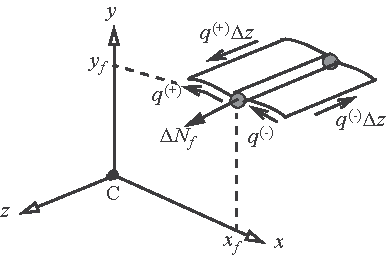
\includegraphics{Figure_3-20.pdf}
\caption{Free body diagram of the stringer.\label{fig3.20}}
\end{wrapfigure}

\noindent That is, the stringer is a longitudinal bar element that does not resist shear. It is modeled as a point on the contour with coordinates $\left[x_{f}\left(s_{f}\right), y_{f}\left(s_{f}\right)\right]$ relative to the centroid, where the contour coordinate of the stringer is denoted by $s_{f}$. Thus, the stringer is mathematically represented as a point on the contour having the attribute of area. See figure~\ref{fig3.20}.

The area and first area moments given by eq.~(\ref{eq3.74}) are modified to account for the cross section with stringers as
\begin{align}
A&=\int_{c} t(s) d s+\hspace*{-3pt}\sum_{\text {stringers }} A_{f} \quad Q_{x}=\int_{c} y(s) t(s) d s+\hspace*{-3pt}\sum_{\text {stringers }} y_{f} A_{f} \nonumber\\
Q_{y} &=\int_{c} x(s) t(s) d s+\sum_{\text {stringers }} x_{f} A_{f}.\label{eq3.133}
\end{align}
Note that first area moments about the centroid are required to satisfy $Q_{x}=Q_{y}=0$. The second area moments about the centroid in eq.~(\ref{eq3.77}) are modified to
\begin{align}
I_{x x}=\int_{c} y^{2} t d s+\sum_{\text {stringers }} y_{f}^{2} A_{f} \quad I_{y y}=\int_{c} x^{2} t d s+\sum_{\text {stringers }} x_{f}^{2} A_{f} \quad
I_{x y}=\int_{c} x y t d s+\sum_{\text {stringers }} x_{f} y_{f} A_{f}. \label{eq3.134}
\end{align}

\vspace*{-1pc}

The material law for extension and bending (\ref{eq3.79}) on page \pageref{eq3.79} remains valid with the geometric properties specified by eqs. (\ref{eq3.133}) and (\ref{eq3.134}). The thermal axial force $N_{T}$ is given by eq.~(\ref{eq3.75}) on page \pageref{eq3.75}, and the thermal bending moments $M_{x T}$ and $M_{y T}$ are given by eq.~(\ref{eq3.78}).

\subsection{Effect of stringers on the shear flow distribution}\label{sec3.10.1}

The shear flow exiting the stringer location is denoted by $q^{(+)}$, the shear flow entering the stringer location by $q^{(-)}$, and the increase in the axial force in the stringer by $\Delta N_{f}$. See figure~\ref{fig3.20}. Sum the forces in the $z$-direction of the free body diagram shown in figure~\ref{fig3.20} to get
\begin{align*}
q\big(s_{f}^{(+)}\big) \Delta z-q\big(s_{f}^{(-)}\big) \Delta z+\Delta N_{f}=0.
\end{align*}
Divide this equilibrium equation by the incremental length $\Delta z$, then let $\Delta z \rightarrow 0$ to get in the limit
\begin{align}\label{eq3.135}
q\left(s_{f}^{(+)}\right)-q\left(s_{f}^{(-)}\right)+\frac{d N_{f}}{d z}=0.
\end{align}
Combine eqs. (\ref{eq3.95}) and (\ref{eq3.97}) to write the shear flow as
\begin{align}\label{eq3.136}
q(s)=q_{0}-\frac{k}{I_{y y}}\left(V_{x}+V_{x T}\right) \bar{Q}_{y}(s)-\frac{k}{I_{x x}}\left(V_{y}+V_{y T}\right) \bar{Q}_{x}(s)-\frac{A(s)}{A} \frac{d N_{T}}{d z}+\int_{0}^{s} \beta \frac{\partial \Delta T}{\partial z} t(s) d s.
\end{align}
Equation (\ref{eq3.89}) was used to identify the derivative of the thermal force in the previous result. Then the jump in the shear flow across the stringer is
\begin{align}
q\left(s_{f}^{(+)}\right)-q\left(s_{f}^{(-)}\right)=&-\left\{\frac{k}{I_{y y}}\left(V_{x}+V_{x T}\right)\left[\bar{Q}_{y}\left(s_{f}^{(+)}\right)-\bar{Q}_{y}\left(s_{f}^{(-)}\right)\right]\right\}-\left\{\frac{k}{I_{x x}}\left(V_{y}+V_{y T}\right)\left[\bar{Q}_{x}\left(s_{f}^{(+)}\right)-\bar{Q}_{x}\left(s_{f}^{(-)}\right)\right]\right\} \nonumber\\[6pt] &-\frac{\left[A\left(s_{f}^{(+)}\right)-A\left(s_{f}^{(-)}\right)\right]}{A} \frac{d N_{T}}{d z}+\left(\int_{s_{f}^{(-)}}^{s_{f}^{(+)}} \beta \frac{\partial \Delta T}{\partial z} t(s) d s\right) .\label{eq3.137}
\end{align}
Note that
\begin{align}\label{eq3.138}
A\left(s_{f}^{(+)}\right)-A\left(s_{f}^{(-)}\right)=A_{f} \quad~\text{and } \quad \int_{s_{f}^{(-)}}^{s_{f}^{(+)}} \beta \frac{\partial \Delta T}{\partial z} t(s) d s=\left.A_{f} \beta \frac{\partial \Delta T}{\partial z}\right|_{s_{f}}.
\end{align}
Under the assumption made to model the stringer $N_{f}=\sigma_{z z} A_{f}$. The axial normal stress in the stringer is given in eq.~(\ref{eq3.83}) on page \pageref{eq3.83}. Thus, $\frac{d N_{f}}{d z}=A_{f} \frac{d \sigma_{z z}}{d z}$. Derivatives of the axial force and bending moments with respect to \textit{z} appearing in $d \sigma_{z z} / d z$ were replaced by equilibrium differential equations (\ref{eq3.53}), (\ref{eq3.55}), and (\ref{eq3.57}), respectively. The result for the derivative of the normal force in the stringer is
\begin{align}\label{eq3.139}
\frac{d N_{f}}{d z}=\frac{k}{I_{y y}}\left(V_{x}+V_{x T}\right) A_{f} \bar{x}_{f}+\frac{k}{I_{x x}}\left(V_{y}+V_{y T}\right) A_{f_{f}} \bar{y}_{f}+\frac{A_{f}}{A} \frac{d N_{T}}{d z}-\left.A_{f} \beta \frac{\partial \Delta T}{\partial z}\right|_{s_{f}}.
\end{align}
Substitute eqs. (\ref{eq3.137}) and (\ref{eq3.139}) into (\ref{eq3.135}) to find
\begin{align}\label{eq3.140}
-\left\{\frac{k}{I_{y y}}\left(V_{x}+V_{x T}\right)\left[\bar{Q}_{y}\left(s_{f}^{(+)}\right)-\bar{Q}_{y}\left(s_{f}^{(-)}\right)-A_{f} \bar{x}_{f}\right]\right\}&-\left\{\frac{k}{I_{x x}}\left(V_{y}+V_{y T}\right)\left[\bar{Q}_{x}\left(s_{f}^{(+)}\right)-\bar{Q}_{x}\left(s_{f}^{(-)}\right)-A_{f} \bar{y}_{f}\right]\right\} \nonumber\\[6pt]
&-\frac{A_{f}}{A} \frac{d N_{T}}{d z}+\frac{A_{f}}{A} \frac{d N_{T}}{d z}+\left.A_{f} \beta \frac{\partial \Delta T}{\partial z}\right|_{s_{f}}-\left.A_{f} \beta \frac{\partial \Delta T}{\partial z}\right|_{s_{f}}=0.
\end{align}
Equation (\ref{eq3.140}) simplifies to
\begin{align}\label{eq3.141}
-\left\{\frac{k}{I_{y y}}\left(V_{x}+V_{x T}\right)\left[\bar{Q}_{y}\left(s_{f}^{(+)}\right)-\bar{Q}_{y}\left(s_{f}^{(-)}\right)-A_{f} \bar{x}_{f}\right]\right\}-\left\{\frac{k}{I_{x x}}\left(V_{y}+V_{y T}\right)\left[\bar{Q}_{x}\left(s_{f}^{(+)}\right)-\bar{Q}_{x}\left(s_{f}^{(-)}\right)-A_{f} \bar{y}_{f}\right]\right\}=0.
\end{align}

\clearpage

\noindent Equation (\ref{eq3.141}) is valid for every choice of the shear actions $\left(V_{x}+V_{x T}\right)$ and $\left(V_{y}+V_{y T}\right)$. Then to satisfy eq.~(\ref{eq3.141}), the coefficients of the shear actions must vanish, which leads to
\begin{align}\label{eq3.142}
\bar{Q}_{y}\left(s_{f}^{(+)}\right)-\bar{Q}_{y}\left(s_{f}^{(-)}\right)-A_{f} \bar{x}_{f}=0 \quad \bar{Q}_{x}\left(s_{f}^{(+)}\right)-\bar{Q}_{x}\left(s_{f}^{(-)}\right)-A_{f} \bar{y}_{f}=0.
\end{align}
Relations (\ref{eq3.84}) and (\ref{eq3.93}) evaluated at $s=s_{f}$ are repeated in the following relations:
\begin{align}\label{eq3.143}
\bar{x}_{f}=x_{f}-n_{x} y_{f} \quad \bar{y}_{f}=y_{f} - n_{y} x_{f} \quad \bar{Q}_{x}\left(s_{f}^{-}\right)=Q_{x}\left(s_{f}^{-}\right)-n_{y} Q_{y}\left(s_{f}^{-}\right) \quad \bar{Q}_{y}\left(s_{f}^{-}\right)=Q_{y}\left(s_{f}^{-}\right)-n_{x} Q_{x}\left(s_{f}^{-}\right).
\end{align}
After substituting the relations (\ref{eq3.143}) into eq.~(\ref{eq3.142}) we get
\begin{align}\label{eq3.144}
Q_{y}\left(s_{f}^{(+)}\right)-Q_{y}\left(s_{f}^{(-)}\right)-A_{f} x_{f}=0, \quad Q_{x}\left(s_{f}^{(+)}\right)-Q_{x}\left(s_{f}^{(-)}\right)-A_{f} y_{f}=0.
\end{align}
Equation (\ref{eq3.144}) shows that the jump in the shear flows exiting and entering the stringer (\ref{eq3.135}) is equivalent to a jump in value of the first area moments across the stringer area.



\section{Closed cross-sectional contour}\label{sec3.11}

Consider a single-cell, closed cross-sectional contour as shown in figure~\ref{fig3.21}. The shear flow acting tangent to the contour is given by eq.~(\ref{eq3.97}) on page \pageref{eq3.97}, where we assume the shear flow from the prescribed change in temperature vanishes. (Refer to the discussion in the paragraph preceding eq.~(\ref{eq3.97}).) Then the shear flow is given~by
\begin{align}\label{eq3.145}
q(s, z)=q_{0}(z)-\frac{k}{I_{y y}} V_{x} \bar{Q}_{y}(s)-\frac{k}{I_{x x}} V_{y} \bar{Q}_{x}(s).
\end{align}
The shear flow is statically equivalent to the shear forces and the torque acting on the cross section. The static equivalence with respect to the shear center given by eq.~(\ref{eq3.40}) on page \pageref{eq3.40} reduces to
{\def\thefigure{3.21}
\begin{figure}[!h]
\centerline{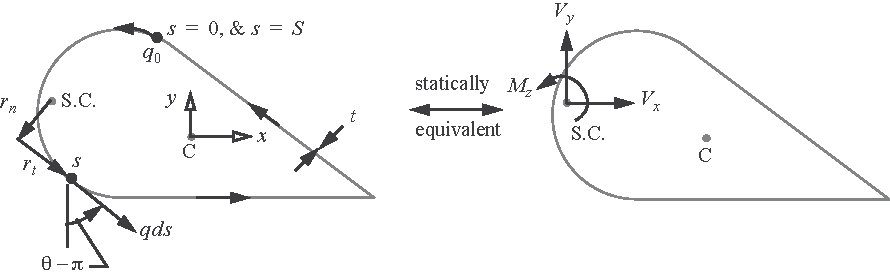
\includegraphics{Figure_3-21.pdf}}
\caption{Static equivalence of the shear flow acting along a closed contour to shear forces and torque.}\label{fig3.21}
\vspace*{-8pt}
\end{figure}}
\begin{align}\label{eq3.146}
V_{x}=\oint(-q \sin \theta) d s \quad V_{y}=\oint(q \cos \theta) d s \quad M_{z}=\oint\left(r_{n} q\right) d s.
\end{align}
(It is assumed that the transverse shear resultant $q_z$ and the twisting moment resultant $m_{zs}$ are small with respect to the shear flow, and therefore are neglected in eq.~(\ref{eq3.40}).) The shear flow formula (\ref{eq3.145}) is the sum of the open section shear flow, eq.~(\ref{eq3.98}), plus a shear flow $q_0$ that is the spatially uniform around the contour.\vadjust{\vspace*{10pt}\pagebreak} If (\ref{eq3.145}) is substituted for the shear flow in the two expressions for the shear forces in (\ref{eq3.146}), it can be shown\footnote{Employ eq. (\ref{eq3.3}) and integrate by parts using the results from eq.~(\ref{eq3.105}).} that we get identities $V_{x}=V_{x}$ and $V_{y}=V_{y}$. That is, the shear flow (\ref{eq3.145}) is statically equivalent to the shear forces $V_x$ and $V_y$. independent of $q_0$. If we substitute the shear flow (\ref{eq3.145}) into the expression for the torque in eq.~(\ref{eq3.146}), then the shear flow $q_0$ can be determined from the torque acting at the shear center. However, the location of the shear center is not known.

Since the location of the centroid is determined before the location of the shear center, consider the torque from the shear flow resolved at the centroid. That is $M_{z C}=\oint r_{n c}(s) q(s) d s$. The coordinate normal to the contour relative to the centroid $r_{n c}(s)$ is determined by the second equation in eq.~(\ref{eq3.11}) on page \pageref{eq3.11}. Substitute the shear flow (\ref{eq3.145}) into the expression for the torque at the centroid to get
\begin{align}\label{eq3.147}
M_{z C}=\oint r_{n c}\left(q_{0}-\frac{k}{I_{y y}} V_{x} \bar{Q}_{y}-\frac{k}{I_{x x}} V_{y} \bar{Q}_{x}\right) d s=q_{0} \oint r_{n c} d s-\frac{k}{I_{y y}} V_{x} \oint r_{n c} \bar{Q}_{y} d s-\frac{k}{I_{x x}} V_{y} \oint r_{n c} \bar{Q}_{x} d s.
\end{align}


\begin{wrapfigure}[10]{R}{149pt}
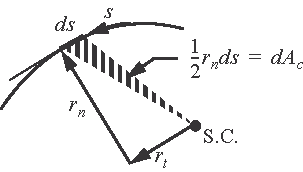
\includegraphics{Figure_3-22.pdf}
\caption{Enclosed area element.\label{fig3.22}}
\end{wrapfigure}


\noindent Let the area enclosed by the contour be denoted by $A_{c}$. As shown in figure~\ref{fig3.22}, the enclosed area is given by
\begin{align}\label{eq3.148}
A_{c}=\frac{1}{2} \oint r_{n} d s=\frac{1}{2} \oint r_{n c} d s.
\end{align}
The two expressions given above for the enclosed area is a consequence of the relation (\ref{eq3.10}) between the normal coordinates $r_{n}$ and $r_{n c}$ when integrated around the closed contour. Solve eq.~(\ref{eq3.147}) for $q_0$ to find
\begin{align}\label{eq3.149}
q_{0}=\frac{M_{z c}}{2 A_{c}}+\frac{k}{2 A_{c} I_{y y}} V_{x} \oint r_{n c} \bar{Q}_{y} d s+\frac{k}{2 A_{c} I_{x x}} V_{y} \oint r_{n c} \bar{Q}_{x}ds.
\end{align}
Substitute the result for $q_0$ from eq.~(\ref{eq3.149}) the into eq.~(\ref{eq3.145}) and denote the resulting expression for this shear flow as $q_C$: the shear flow with respect to the centroid. The result for $q_C$ is written as
\begin{align}\label{eq3.150}
q_{C}(s, z)=\frac{M_{z C}(z)}{2 A_{c}}-F_{x c}(s) V_{x}(z)-F_{y c}(s) V_{y}(z),
\end{align}
where the shear flow distribution functions relative to the centroid are defined by
\begin{align}\label{eq3.151}
F_{x c}(s)=\frac{k}{I_{y y}}\left[\bar{Q}_{y}(s)-\frac{1}{\left(2 A_{c}\right)} \oint r_{n c}(s) \bar{Q}_{y}(s) d s\right] \quad F_{y c}(s)=\frac{k}{I_{x x}}\left[\bar{Q}_{x}(s)-\frac{1}{\left(2 A_{c}\right)} \oint r_{n c}(s) \bar{Q}_{x}(s) d s\right].
\end{align}
We have used all the conditions of static equivalence to determine the shear flow. with respect to the centroid. Thus, it is a statically indeterminate problem to find the expression for shear flow relative to the shear center, as well as the location of the shear center in the cross section. The additional relation we need is a constitutive relation between the twist per unit length $d \phi_{z} / d z$ and the shear flow $q$.

\subsection{Twist per unit longitudinal length}\label{sec3.11.1}

The shear strain $\gamma_{z s}$ evaluated at the contour from eq.~(\ref{eq3.31}) on page \pageref{eq3.31} is
\begin{align}\label{eq3.152}
\gamma_{z s}(s, z)=\psi_{x}(z) \frac{d x}{d s}+\psi_{y}(z) \frac{d y}{d s}+r_{n}(s) \frac{d \phi_{z}}{d z} \quad~\text{at } \quad \zeta=0,
\end{align}

\vspace*{-1pc}\pagebreak

\noindent where eq.~(\ref{eq3.3}) was used to write the trigonometric functions in terms of the derivatives of the contour coordinate functions. Integrate the shear strain (\ref{eq3.152}) around the closed contour to get\vspace*{-2pt}
\begin{align}\label{eq3.153}
\oint\!\gamma_{z s} d s=\psi_{x}(z) \underbrace{\oint{\frac{d x}{d s}} d s}_{=\;0}+\psi_{y}(z) \underbrace{\oint{\frac{d y}{d s} d s}}_{=\;0}
+\underbrace{\oint r_{n} d s}_{=\;2 A_{c}} \frac{d \phi_{z}}{d z}.
\end{align}

\vspace*{-14pt}

\noindent Continuity of the contour and the eq.~(\ref{eq3.148}) for the enclosed area results in\vspace*{-2pt}
\begin{align*}
\frac{d \phi_{z}}{d z}=\frac{1}{2 A_{c}} \oint \gamma_{z s} d s.
\end{align*}

\vspace*{-14pt}

\noindent Hooke's law relates the shear strain to the shear stress by $\gamma_{z s}=\sigma_{z s} / G$, where $G$ is the shear modulus of the material. In torsion of a closed cross-sectional contour the shear stress is assumed uniform through the thickness of the wall. Hence, the shear stress is determined by the shear flow divided by the thickness of the wall, or $\sigma_{z s}=q / t$. Substitute $\gamma_{z s}=q /(G t)$ into the equation for the twist per unit length to get.
\begin{align}\label{eq3.154}
\fbox{$\displaystyle\frac{d \phi_{z}}{d z}=\frac{1}{2 A_{c}} \oint\left(\frac{q}{G t}\right) d s$}.
\end{align}

\subsection{Location of the shear center and the final expression for the shear flow}\label{sec3.11.2}

Substitute eq.~(\ref{eq3.150}) for the shear flow in eq.~(\ref{eq3.154}) to find
\begin{align}\label{eq3.155}
\frac{d \phi_{z}}{d z}=\frac{M_{z C}}{4 A_{c}^{2}} \oint \frac{d s}{G t}-\frac{V_{x}}{2 A_{c}} \oint \frac{F_{x c}}{G t} d s-\frac{V_{y}}{2 A_{c}} \oint \frac{F_{y c}}{G t} d s.
\end{align}
\noindent The torque $M_{zc}$ and shear forces $V_x$ and $V_y$ are resolved at the centroid. We can find a statically equivalent torque and force system resolved at the shear center: Simply add and subtract the shear forces at the shear center which does not change static equivalence as shown in figure~\ref{fig3.23}(a). The upward force $V_y$ at point $C$ and the downward force $V_y$ at S.C. form a clockwise couple $x_{sc} V_{y}$ and no net vertical force. Similarly, rightward force $V_x$ at point $C$ and the leftward force $V_x$ at the S.C. form a counterclockwise couple $y_{sc} V_{x}$ and no net horizontal force. The total counterclockwise torque in the cross section is $M_{z c}-x_{s c} V_{y}+y_{s c} V_{x}$. Formulating these couples leave forces $V_x$ and $V_y$ at the shear center as shown in part (b) of figure~\ref{fig3.23} and a counterclockwise torque. Thus, the torque at the shear center must be
\begin{align}\label{eq3.156}
M_{z}=M_{z C}-x_{s c} V_{y}+y_{s c} V_{x}.
\end{align}

{\def\thefigure{3.23}
\processfigure[H]{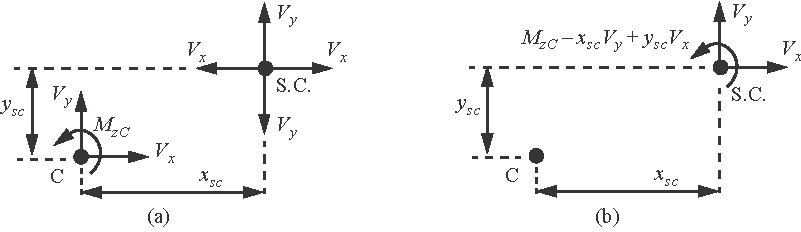
\includegraphics{Figure_3-23.pdf}
}{\caption{The method to move the shear forces from the centroid to the shear center while maintaining static equivalence.\label{fig3.23}}}}

\noindent Solve eq.~(\ref{eq3.156}) for the torque at the centroid and substitute the result for $M_{zC}$ into eq.~(\ref{eq3.155}) to get
\begin{align}\label{eq3.157}
\frac{d \phi_{z}}{d z}=\frac{M_{z}}{4 A_{c}^{2}} \oint \frac{d s}{G t}-\left[\frac{y_{s c}}{4 A_{c}^{2}} \oint \frac{d s}{G t}+\frac{1}{2 A_{c}} \oint \frac{F_{x c}}{G t} d s\right] V_{x}+\left[\frac{x_{s c}}{4 A_{c}^{2}} \oint \frac{d s}{G t}-\frac{1}{2 A_{c}} \oint \frac{F_{y c}}{G t} d s\right] V_{y}.
\end{align}
At the shear center the twist per unit length depends on the torque resolved at the shear center and not on the shear forces. In other words, the shear forces acting at the shear center do not contribute to torsion. This requirement means the coefficients of the shear forces in eq.~(\ref{eq3.157}) must vanish. Equating these coefficients to zero determines the coordinates of the shear center relative to the centroid as
\begin{align}\label{eq3.158}
x_{s c}=\left[\frac{2 A_{c}}{\oint \frac{d s}{G t}} \oint\left(\frac{F_{y c}(s)}{G t}\right) d s\right] \quad y_{s c}=-\left[\frac{2 A_{c}}{\oint \frac{d s}{G t}} \oint\left(\frac{F_{x c}(s)}{G t}\right) d s\right].
\end{align}
Equation (\ref{eq3.157}) reduces to the form
\begin{align}\label{eq3.159}
\frac{d \phi_{z}}{d z}=\frac{M_{z}}{(G J)_{\mathrm{eff}}},
\end{align}
where the effective torsional stiffness is
\begin{align}\label{eq3.160}
(G J)_{\mathrm{eff}}=\frac{4 A_{c}^{2}}{\oint \frac{d s}{G t}}.
\end{align}
If the shear modulus is uniform around the contour, then
\begin{align}\label{eq3.161}
\frac{d \phi_{z}}{d z}=\frac{M_{z}}{G J}\mbox{ and the torsion constant is }J=\frac{4 A_{c}^{2}}{\oint \frac{d s}{t}}.
\end{align}

Substitute the solution for the torque at the centroid from eq.~(\ref{eq3.156}) into the expression for the shear flow in eq.~(\ref{eq3.150}). In the process, we drop the ``C'' subscript on $q_C$ to indicate that we are formulating the shear flow relative to the shear center. The result is
\begin{align}\label{eq3.162}
q=\frac{M_{z}+x_{s c} V_{y}-y_{s c} V_{x}}{2 A_{c}}-F_{x c}(s) V_{x}(z)-F_{y c}(s) V_{y}(z).
\end{align}
Equation (\ref{eq3.162}) is written in the form
\begin{align}\label{eq3.163}
\fbox{$\displaystyle q(s, z)=\frac{M_{z}(z)}{2 A_{c}}-F_{x}(s) V_{x}(z)-F_{y}(s) V_{y}(z)$},
\end{align}
where the shear flow distribution functions relative to the shear center are defined by
\begin{align}\label{eq3.164}
F_{x}(s)=\frac{y_{s c}}{2 A_{c}}+F_{x c}(s) \quad F_{y}(s)=-\left(\frac{x_{s c}}{2 A_{c}}\right)+F_{y c}(s).
\end{align}

\vspace*{-1pc}

 In \textbf{pure torsion} only torque $M_z$ acts on the section, and the shear terms in eq.~(\ref{eq3.163}) vanish. Then in pure torsion the shear flow is spatially uniform around the contour and leads to
\begin{align}\label{eq3.165}
q=\frac{M_{z}}{2 A_{c}} \quad~\text{or } \quad M_{z}=2 A_{c} q.
\end{align}
Equation (\ref{eq3.165}) is called \textbf{Bredt's formula}, or the Bredt-Batho formula, and it relates the torque to the uniform shear flow in a single-cell section subject to torsion only.

\clearpage

\begin{example*}[A single-cell cross section stiffened by axial stringers]\label{ex3.4}\setcounter{equation}{0}\def\theequation{\alph{equation}}A uniform bar of length $L$ with a closed, cross-sectional contour is stiffened by four axial stringers. The configuration and the associated nomenclature is shown in figure~\ref{fig3.24}(a), where the $X$-axis is an axis of symmetry. The areas of the stringer flanges are denoted by $A_{f1}$ and $A_{f2}$, and the wall thickness $t$ is uniform along the entire contour. As shown in figure~\ref{fig3.24}(b), the contour is divided into four branches. Branch 1 is a semicircle segment of radius \textit{a} between the lower stringer $A_{f1}$ and the upper stringer $A_{f1}$ of length $a\pi$, branch 2 is the horizontal\break segment between upper stringer $A_{f1}$ and upper stringer $A_{f2}$ of length $b$, branch 3 is the vertical segment\break between the upper stringer $A_{f2}$ and the lower stringer $A_{f2}$ of length 2$a$, and branch 4 is the horizontal segment~bet\-ween~lower stringer $A_{f2}$ and lower stringer $A_{f1}$ of length $b$. Dimensional data are
\begin{align*}
a=6~\text{in. } \quad b=7~\text{in. } \quad t=0.03~\text{in.} \quad A_{f 1}=0.30~\text{in.}^{2} \quad~\text{and } \quad A_{f 2}=0.70~\text{in.}^{2}
\end{align*}
The numerical results presented in the solution of this example were performed in \textit{Mathematica}.
{\def\thefigure{3.24}
\processfigure[H]{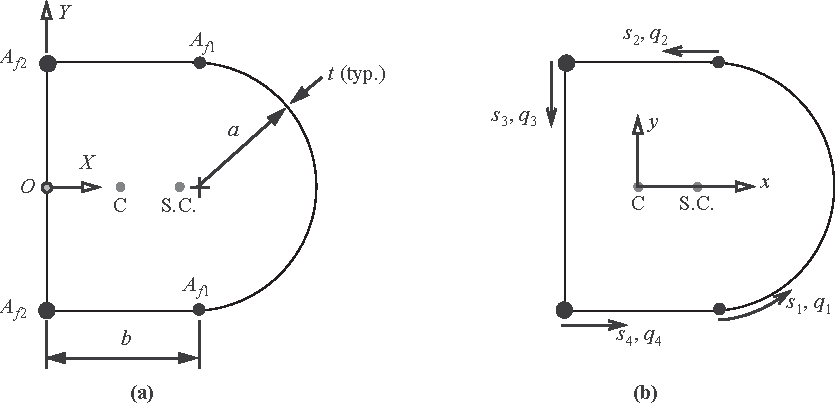
\includegraphics{Figure_3-24.pdf}
}{\caption{Single-cell cross section. (a) Geometry. (b) Branch coordinates and associated shear flows.\label{fig3.24}}}}
\begin{enumerate}
\item[a)] Determine the location of the centroid (C) and the second area moments $I_{x x}$ and $I_{y y}$.

\item[b)] Determine the shear flow distribution functions $F_{x c}(s)$ and $F_{y c}(s)$ with respect to the centroid.

\item[c)] Determine the location of the shear center (S.C.) relative to the centroid.%\vspace*{-4pt}
\end{enumerate}

\subsubsection{Solution to part (a).} Take the origin of the \textit{X-Y} system at point $O$, the center of the vertical web. The parametric equations of the contour in each branch are listed in table \ref{tab3.2},

The area $A$ of the cross section is given by%\enlargethispage{-2\baselineskip}
\begin{align}\label{ex3.4a}
A=\sum_{i=1}^{4} \int_{0}^{\left(s_{i}\right)_{\max }} t d s_{i}+2 A_{f 1}+2 A_{f 2}=3.34549~\mathrm{in.}^{2}.
\end{align}

\vspace*{5pt}

\clearpage

\begin{table}%Table 3.2
\processtable{Parametric equations of the contour in example \ref{ex3.4}\label{tab3.2}}
{\tabcolsep=12pt\begin{tabular}{@{}llll@{}}
\toprule
\colhead{Branch} & \colhead{$X_{i}=$} & \colhead{$Y_{i}=$} & \colhead{Range}\\
\midrule
$i=1$ & $b+a \sin \left(s_{1} / a\right)$ & $-a \cos \left(s_{1} / a\right)$ & $0 \leq s_{1} \leq a \pi$\\
$i=2$ & $b-s_{2}$ & $a$ & $0 \leq s_{2} \leq b$\\
$i=3$ & $0$ & $a-s_{3}$ & $0 \leq s_{3} \leq 2 a$\\
$i=4$ & $s_{4}$ & $-a$ & $0 \leq s_{4} \leq b$\\\botrule
\end{tabular}}{}
\vspace*{-1pc}
\end{table}\allowdisplaybreaks

\noindent Since the cross section is symmetric about the $X$-axis, the centroid is located on this axis of symmetry. To locate the centroid we only need to compute the first area moment about the $Y$-axis. The first area moment $Q_{Y}$ is given~by
\begin{align}\label{ex3.4b}
Q_{Y}=\sum_{i=1}^{4} \int_{0}^{\left(s_{i}\right)_{\max }} X_{i}\left(s_{i}\right) t d s_{i}+X_{1}(0) A_{f 1}+X_{2}(0) A_{f 1}+X_{3}(0) A_{f 2}+X_{4}(0) A_{f 2}=11.7884~\text{in.}^{3}.
\end{align}
The centroid coordinate is $X_{c}=Q_{Y} / A=3.52367$ in., and by symmetry $Y_{c}=0$. The Cartesian coordinates $x$ and $y$ with origin at the centroid are related to coordinates $X$ and $Y$ by
\begin{align}\label{ex3.4c}
x_{i}\left(s_{i}\right)=X_{i}\left(s_{i}\right)-X_{c}\mbox{ and }y_{i}\left(s_{i}\right)=Y_{i}\left(s_{i}\right)-Y_{c}=Y_{i}\left(s_{i}\right),\quad i=1,2,3,4.
\end{align}
From eq.~(\ref{eq3.77}) the second area moment about the $x$- and $y$-axes are given by
\begin{gather}\label{ex3.4d}
I_{x x}=\sum_{i=1}^{4} \int_{0}^{\left(s_{i}\right)_{\max }} y_{i}^{2}\left(s_{i}\right) t d s_{i}+y_{1}^{2}(0) A_{f 1}+y_{2}^{2}(0) A_{f 1}+y_{3}^{2}(0) A_{f 2}+y_{4}^{2}(0) A_{f 2}=101.619~\text{in.}^{4}\mbox{, and}\\[6pt]
I_{y y}=\sum_{i=1}^{4} \int_{0}^{\left(s_{i}\right)_{\max }} x_{i}^{2}\left(s_{i}\right) t d s_{i}+x_{1}^{2}(0) A_{f 1}+x_{2}^{2}(0) A_{f 1}+x_{3}^{2}(0) A_{f 2}+x_{4}^{2}(0) A_{f 2}=62.8491~\text{in.}^{4}.\label{ex3.4e}
\end{gather}
The product area moment $I_{x y}=0$ since the $x$-axis is an axis of symmetry of the cross-sectional area.

\vspace*{-6pt}
%\enlargethispage{-1\baselineskip}

\subsubsection{Solution to part (b).} The first area moments about the $x$-axis for segments of each branch including~string\-ers~are
\begin{gather}\label{ex3.4f}
Q_{x 1}\left(s_{1}\right)=y_{1}(0) A_{f 1}+\int_{0}^{s_{1}} y_{1}\left(s_{1}\right) t d s_{1}=-1.8\left[1+\sin \left(s_{1} / 6\right)\right] \quad 0 \leq s_{1} \leq 6 \pi,\\[6pt]
Q_{x 2}\left(s_{2}\right)=Q_{x 1}(6 \pi)+y_{2}(0) A_{f 1}+\int_{0}^{s_{2}} y_{2}\left(s_{2}\right) t d s_{2}=0.18 s_{2} \quad 0 \leq s_{2} \leq 7~\textrm{in.},\label{ex3.4g}\\[6pt]
Q_{x 3}\left(s_{3}\right)=Q_{x 2}(7)+y_{3}(0) A_{f 2}+\int_{0}^{s_{3}} y_{3}\left(s_{3}\right) t d s_{3}=5.46+0.18 s_{3}-0.015 s_{3}^{2} \quad 0 \leq s_{3} \leq 12~\textrm{in.},\label{ex3.4h}\\[6pt]
Q_{x 4}\left(s_{4}\right)=Q_{x 3}(12)+y_{4}(0) A_{f 2}+\int_{0}^{s_{4}} y_{4}\left(s_{4}\right) t d s_{4}=1.26-0.18 s_{4} \quad 0 \leq s_{4} \leq 7~\text{in.}.\label{ex3.4i}
\end{gather}
As a check on the computation we evaluate $Q_{x 4}(7)$ to find $Q_{x 4}(7)=-2.2 \times 10^{-16} \sim 0$. The value of $Q_{x 4}(7)$ equals the first area moment about the $x$-axis through the centroid of the entire cross section, which vanishes by the definition of the centroid. The first area moments about the $y$-axis for segments of each branch including stringers~are\pagebreak
\begin{gather}\label{ex3.4j}
Q_{y 1}\left(s_{1}\right)=x_{1}(0) A_{f 1}+\int_{0}^{s_{1}} x_{1}\left(s_{1}\right) t d s_{1}=2.1229+0.10429 s_{1}-1.08 \cos \left(s_{1} / 6\right) \quad 0 \leq s_{1} \leq 6 \pi,\\[6pt]
Q_{y 2}\left(s_{2}\right)=Q_{y 1}(6 \pi)+x_{2}(0) A_{f 1}+\int_{0}^{s_{2}} x_{2}\left(s_{2}\right) t d s_{2}=6.21161+0.10429 s_{2}-0.015 s_{2}^{2} \quad 0 \leq s_{2} \leq 7~\text{in.},\label{ex3.4k}\\[6pt]
Q_{y 3}\left(s_{3}\right)=Q_{y 2}(7)+x_{3}(0) A_{f 2}+\int_{0}^{s_{3}} x_{3}\left(s_{3}\right) t d s_{3}=3.74007-0.10571 s_{3} \quad 0 \leq s_{3} \leq 12~\mathrm{ in.},\label{ex3.4l}\\[6pt]
Q_{y 4}\left(s_{4}\right)=Q_{y 3}(12)+x_{4}(0) A_{f 2}+\int_{0}^{s_{4}} x_{4}\left(s_{4}\right) t d s_{4}=0.00497169-0.10571 s_{4}+0.015 s_{4}^{2} \quad 0 \leq s_{4} \leq 7~\text{in.}.\tag{d}
\end{gather}
We evaluate $Q_{y 4}(7)$ to find $Q_{y 4}(7)=-1.6 \times 10^{-15} \sim 0$, which is as expected for a correct computation of the first area moment functions $Q_{y i}\left(s_{i}\right)$, $i=1,2,3,4$. From eq.~(\ref{eq3.11}) on page \pageref{eq3.11}, the results for the normal coordinate functions with respect to the centroid for each branch are
\begin{align}\label{ex3.4m}
r_{n c 1}=6+3.347633 \sin \left(s_{1} / 6\right) \quad r_{n c 2}=6 \quad r_{n c 3}=3.52367=X_{c} \quad r_{n c 4}=6.
\end{align}
The area enclosed by the contour is
\begin{align}\label{ex3.4n}
A_{c}=\frac{1}{2} \sum_{i=1}^{4} \int_{0}^{\left(s_{i}\right)_{\max }} r_{n c i} d s_{i}=140.549~\text{in.}^{2}.
\end{align}
Since the product area moment $I_{x y}=0$, eq.~(\ref{eq3.81}) gives $n_{x}=0$, $n_{y}=0$, and $k=1$. Moreover, from eq.~(\ref{eq3.93}) we find $\bar{Q}_{x}(s)=Q_{x}(s)$ and $\bar{Q}_{y}(s)=Q_{y}(s)$. Thus, the expressions for the shear flow distribution functions $F_{x c}(s)$ and $F_{y c}(s)$ in eq.~(\ref{eq3.151}) simplify. For each branch the shear flow distribution functions are given by
\begin{gather}\label{ex3.4o}
F_{x c i}\left(s_{i}\right)=\left[Q_{y i}\left(s_{i}\right)-\left(\frac{1}{2 A_{c}}\right) \sum_{i=1}^{4} \oint\left[r_{n c i}\left(s_{i}\right)\right] Q_{y i}\left(s_{i}\right) d s_{i}\right] \frac{1}{I_{y y}}\mbox{, and}\\[6pt]
F_{y c i}\left(s_{i}\right)=\left[Q_{x i}\left(s_{i}\right)-\left(\frac{1}{2 A_{c}}\right) \sum_{i=1}^{4} \oint\left[r_{n c i}\left(s_{i}\right)\right] Q_{x i}\left(s_{i}\right) d s_{i} \right]\frac{1}{I_{x x}}.\label{ex3.4p}
\end{gather}
Evaluation of the following\enlargethispage{-1\baselineskip} terms in the previous equations are
\begin{align}\label{ex3.4q}
\left(\frac{1}{2 A_{c}}\right)\sum_{i=1}^{4} \oint r_{n c i}\left(s_{i}\right) Q_{y i}\left(s_{i}\right) d s_{i}=3.10581~\text{in.}^{3} \quad\left(\frac{1}{2 A_{c}}\right) \sum_{i=1}^{4} \oint r_{n c i}\left(s_{i}\right) Q_{x i}\left(s_{i}\right) d s_{i}=-0.330117~\text{in.}^{3}.
\end{align}
The results for shear flow distribution functions $F_{x c i}\left(s_{i}\right)$ are
\begin{gather}\label{ex3.4r}
F_{x c 1}\left(s_{1}\right)=-0.0156392+0.00165937 s_{1}-0.017184 \cos \left(s_{1} / 6\right) \quad 0 \leq s_{1} \leq 6 \pi,\\[4pt]
F_{x c 2}\left(s_{2}\right)=0.494169+0.00165937 s_{2}-0.000238667 s_{2}^{2} \quad 0 \leq s_{2} \leq 7~\text{in.},\label{ex3.4s}\\[4pt]
F_{x c 3}\left(s_{3}\right)=0.0100918-0.00168197 s_{3} \quad 0 \leq s_{3} \leq 12~\text{in.}\mbox{, and}\label{ex3.4t}\\[4pt]
F_{x c 4}\left(s_{4}\right)=-0.0493378-0.00168197 s_{4}+0.000238667 s_{4}^{2} \quad 0 \leq s_{4} \leq 7~\text{in.}\label{ex3.4u}
\end{gather}
The results for shear flow distribution functions $F_{y c i}\left(s_{i}\right)$ are
\begin{gather}
F_{y c 1}\left(s_{1}\right)=-0.0144647-0.010628 \sin \left(s_{1} / 6\right) \quad 0 \leq s_{1} \leq 6 \pi,\label{ex3.4v}\\
F_{y c 2}\left(s_{2}\right)=0.00324859+0.00177133 s_{2} \quad 0 \leq s_{2} \leq 7~\text{in.},\label{ex3.4w}\\
F_{y c 3}\left(s_{3}\right)=0.0569788+0.00177133 s_{3}-0.000147611 s_{3}^{2} \quad 0 \leq s_{3} \leq 12~\text{in.}\mbox{, and}\label{ex3.4x}\\
F_{y c 4}\left(s_{4}\right)=0.0156479-0.00177133 s_{4} \quad 0 \leq s_{4} \leq 7~\text{in}.\label{ex3.4y}
\end{gather}
The dimensional unit of each shear flow distribution function is $\text { in.}{}^{-1}$

\subsubsection{Solution to part c.} The $x$-coordinate of the shear center is given by eq.~(\ref{eq3.158}). First evaluate the following integral that appears in the denominator of (\ref{eq3.158}):
\begin{align}\label{ex3.4z}
\oint \frac{d s}{G t}=\frac{1}{G t} \sum_{i=1}^{4}\left(s_{i}\right)_{\max }=\frac{1,494.99}{G}.
\end{align}
From (\ref{eq3.158}) the coordinates of the shear center with respect to the centroid are
\begin{align}
x_{s c}&=\frac{2 A_{c}}{\oint{\frac{d s}{Gt}}}\sum^4_{i=1}
\int_{0}^{\left(s_{i}\right)_{\max }}  \frac{F_{y c i}\left(s_{i}\right)}{G t} d s_{i}=2.8727~\mathrm{in.}\mbox{, and }
y_{s c}\nonumber\\
&=-
\left[\frac{2A_{c}}{\oint{\frac{d s}{G t}}} \sum^4_{i=1}
\int^{\left(s_{i}\right)_{\max}}_{0}
\frac{F_{x c i}\left(s_{i}\right)}{G t} d s_{i}\right]=-1.3 \times 10^{-15}~\text{in } \sim 0.\tag{aa}
\end{align}
This result for $y_{\textit{sc}}$ is expected since the shear center lies on an axis of symmetry, and the $x$-axis is the axis of symmetry for the cross section. From eq.~(\ref{eq3.164}) the shear flow distribution functions with respect to the shear center are $F_{x i}\left(s_{i}\right)=F_{x c i}\left(s_{i}\right)$.

We record below for later use the remaining shear flow distribution functions with respect to the shear center, which are determined from eq.~(\ref{eq3.164}).
\begin{gather}
F_{y 1}\left(s_{1}\right)=-0.0246843-0.010628 \sin \left(s_{1} / 6\right) \quad 0 \leq s_{1} \leq 6 \pi\tag{ab} \label{eq3.4.ab}\\
F_{y 2}\left(s_{2}\right)=-0.00697102+0.00177133 s_{2} \quad 0 \leq s_{2} \leq 7~\text{in.}\tag{ac} \label{eq3.4.ac}\\
F_{y 3}\left(s_{3}\right)=0.0467592+0.00177133 s_{3}-0.000147611 s_{3}^{2} \quad 0 \leq s_{3} \leq 12~\text{in.}\tag{ad} \label{eq3.4.ad}\\
F_{y 4}\left(s_{4}\right)=0.00542827-0.00177133 s_{4} \quad 0 \leq s_{4} \leq 7~\mathrm{in}. \tag{ae} \label{eq3.4.ae}
\end{gather}
\end{example*}

\vspace*{-2pc}

\begin{thebibliography}{}
\bibitem{}
Fung, Y. C.\enlargethispage{-1\baselineskip} \textbf{\textit{Foundations of Solid Mechanics}}. Englewood Cliffs, NJ: Prentice-Hall, Inc., 1965, p. 390.

\bibitem{}
Gjelsvik, Atle. \textbf{\textit{The Theory of Thin Walled Bars}}. New York: John Wiley \& Sons, 1981.

\bibitem{}
Goldstein, H. \textbf{\textit{Classical Mechanics}}. Reading MA: Addison Wesley Publishing Inc., 1950, p.~128.\label{Goldstein}

\bibitem{}
Oden, J. T., and E. A. Ripperger, E. A. \textbf{\textit{Mechanics of Elastic Structures}}, 2d ed. New York: Hemisphere Publishing Corporation, New York, 1981, p.~46.

\bibitem{}
Thornton, Earl, A. \textbf{\textit{Thermal Structures for Aerospace Applications.}} Reston VA: American Institute of Aeronautics and Astronautics, Inc., 1996, Chapters 1 and 2, and p. 51.

\bibitem{}
Vasiliev, Valery, V. \textbf{Mechanics of Composite Structures}. Edited by Robert M. Jones, DC: Taylor \& Francis, 1993, p.~205.

\bibitem{}
Vasiliev, Valery V., and Evgeny V. Morozov. \textbf{\textit{Advanced Mechanics of Composite Materials and Structural Elements}}, 3d ed., Waltham, MA: Elsevier, 2013, Chapter 10.
\end{thebibliography}

\clearemptydoublepage

\end{document} 